\chapter{Apéndice del Capítulo \ref{chapter:BIN}}


%\section{Comité de ética}
%Los experimentos fueron aprobados por el comité de ética: Comité d’Ethique pour la Recherche, CER, de l’Université Paris Saclay. Los participantes dieron su consentimiento por escrito para participar y se les pagó por su participación.

\section{Participantes}

%Twenty-eight healthy volunteers (Mage = 24.3, SD = 3.2, 16 women) participated in experiment 1, twenty in experiment 2 (Mage = 26.5, SD = 9.5, 15 women), thirty-two in experiment 3 (Mage = 27.4, SD = 5.3, 21 women), twenty-three in experiment 4 (Mage = 23.4, SD = 4.5, 18 women) and eighteen in experiment 5 (Mage = 25.5, SD = 5.7, 15 women). They all gave written consent to participate and were paid for their participation. In experiment 1, all participants performed the subjective complexity rating task but, due to time constraints, seven of them performed only 6 out of the 10 independent short sessions of deviance detection.

Veintiocho voluntarios sanos (Prom. edad = $24.3$, $S.D. = 3.2$, 16 mujeres) participaron en el experimento 1, veinte en el experimento 2 ( Prom. edad = $26.5$, $S.D. = 9.5$, 15 mujeres), treinta y dos en el experimento 3 ( Prom. edad = $27.4$, $S.D. = 5.3$, 21 mujeres), veintitrés en el experimento 4 ( Prom. edad = $23.4$, $S.D. = 4.5$, 18 mujeres) y dieciocho en el experimento 5 ( Prom. edad = $25.5$, $S.D. = 5.7$, 15 mujeres) . En el experimento 1, todos los participantes realizaron la tarea de calificación de complejidad subjetiva pero, debido a limitaciones de tiempo, siete de ellos realizaron solo 6 de las 10 sesiones cortas independientes de detección de desviación.

\section{Estimulos}

%Auditory binary sequences used in all five experiments were composed of an alternation of low pitch and high pitch tones. Each stimulus was a complex tone synthesized with the superimposition of four sine waves. Sound frequencies were chosen to correspond to musical notes: 494, 740, 988 and 1480Hz (i.e. B, F#, B, F#) for the low pitch tone, and 622, 932, 1245 and 1865Hz (i.e. D#, Bb, D#, Bb) for the high pitch tone. The two complex tones were randomly assigned to items A and B for each experimental session. Thus, stimulus attribution changed from one sequence to the next and from one participant to the next but was kept constant for a given sequence in a given participant. In addition, one lower pitch tone (415, 622, 831 and 1245Hz) and one higher pitch tone (740, 1109, 1480 and 2217Hz) were synthesized, to be used as easy-to-detect súper-deviant (or C) stimuli in experiments 1 and 2. All tones were 50 ms long, with 5 ms initial and final ramp. Inter-stimulus interval (ISI) was 200 ms. 

Las secuencias binarias auditivas utilizadas en los cinco experimentos estaban compuestas por una alternancia de tonos graves y agudos. Cada estímulo era un tono complejo sintetizado con la superposición de cuatro ondas sinusoidales. Las frecuencias de sonido se eligieron para corresponder a las notas musicales: 494, 740, 988 y 1480Hz (es decir, B, F\#, B, F\#) para el tono de tono bajo y 622, 932, 1245 y 1865Hz (es decir, D\#, Bb, D\#, Bb) para el tono agudo. Los dos tonos complejos se asignaron aleatoriamente a los elementos A y B para cada sesión experimental. Por lo tanto, la atribución de estímulo cambió de una secuencia a la siguiente y de un participante al siguiente, pero se mantuvo constante para una secuencia determinada en un participante determinado. Además, se sintetizaron un tono más bajo (415, 622, 831 y 1245Hz) y un tono más alto (740, 1109, 1480 y 2217Hz), para ser utilizados como estímulos súper-desviados (o C) fáciles de detectar en los experimentos 1 y 2. Todos los tonos fueron de 50ms de duración, con transiciones iniciales y finales de 5ms. El intervalo entre estímulos (ISI) fue de 200ms.

%Ten 16-items long sequential patterns were chosen for experiment 1 (see Figure 2), which were all composed of the same number of items (8 As, 8 Bs), giving a total sequence duration of 3800 ms. The first four sequential patterns, of lowest complexity, followed the simple algebraic pattern (AnBn)x: (AB)8, (A2B2)4, (A4B4)2 and A8B8. The period of these sequences differed (2, 4, 8 and 16 tones), but the complexity was identical (LoT complexity = 6).  Although the shortest description formula did not necessarily conform to our intuitive AnBn notation (i.e., [[+0]^16<b>], [[[+0]^2]^8<b>], [[[+0]^4]^4<b>], and [[[+0]^8]^2<b>], respectively), they are indeed all represented with a formula containing 2 instructions and 2 digits. The other 6 sequences had LoT complexity values ranging from 12 to 23. Half of them were periodic (period of 8).

Se eligieron diez patrones secuenciales largos de 16 elementos para el experimento 1 (ver Figura~\ref{PlosBIO-F2}), todos compuestos por el mismo número de elementos (8 As y 8 Bs), dando una duración total de secuencia de 3800ms. Los primeros cuatro patrones secuenciales, de menor complejidad, siguieron el patrón algebraico simple $(A^nB^n)^x$: $(AB)^8$ , $(A^2B^2)^4$, $(A^4B^4)^2$ y $(A^8B^8)$. El período de estas secuencias fue diferente (2, 4, 8 y 16 tonos), pero la complejidad fue idéntica (\mdlbin = 6). Aunque la fórmula de descripción más corta no se ajustaba necesariamente a nuestra notación intuitiva $A^nB^n$ (es decir, $[[+0]^{16}<b>]$, $[[[+0]^2]^ 8 <b>]$, $[[ [+0] ^ 4] ^ 4 <b>]$ y $[[[+0] ^ 8] ^ 2 <b>]$, respectivamente), todos están representados con una fórmula que contiene 2 instrucciones y 2 dígitos. Las otras 6 secuencias tenían valores de complejidad de LoT que iban de 12 a 23. La mitad de ellas eran periódicas (período de 8).

%In experiment 2, twelve 12-items long different sequential patterns, each composed of 6 As and 6 Bs were presented to each participant (Figure 4). Sequence duration was 2800 ms. In experiment 3, thirty-five 8-items long different sequential patterns, each composed of 4 As and 4 Bs, were used (see Fig. S3), i.e. all possible 8-element-long binary combinations that contained the same number of As and Bs. Sequence duration was 1800 ms. In experiment 4, thirty-two 6-items long different sequential patterns were used (see Fig. S4), representing all 25 types of 6-element sequences (given that the labelling of As and Bs is arbitrary, sequences such ABABAB and BABABA were considered identical). Note that, in this case, the proportion of As vs. Bs varied across sequences. Sequence duration was 1300 ms. In experiment 5, fifteen 8-items long sequential patterns were used (see Fig. S7). All were previously used in experiment 2. They were selected based on their LoT complexity, in order to preserve a large and homogenous distribution of complexity values. The same sequences were presented to participants in auditory and visual forms (in different blocks). Auditory sequences were composed of the same two complex tones as in the previous experiments. Visual sequences were composed of two colored Gabor patches presented in the center of the screen (a red Gabor patch with 45° orientation, and a green patch with 135° orientation). Stimulus duration was 200 ms with 200 ms inter-stimulus interval in both modalities. Sequence duration was 3000 ms. 

En el experimento 2, doce patrones de secuencias de 12 elementos, cada uno compuesto de 6 As y 6 Bs se presentaron a cada participante (Figura~\ref{PlosBIO-F4}). La duración de la secuencia fue de 2800ms. En el experimento 3, treinta y cinco patrones de secuencias de 8 elementos, cada uno compuesto de 4 As y 4 Bs, se utilizaron (ver Figura~\ref{PlosBIO-S3}), es decir, todas las posibles combinaciones de 8 elementos binario que contienen el mismo número de As y Bs. La duración de la secuencia fue de 1800ms. En el experimento 4, treinta y dos patrones de secuencia de 6 elementos se utilizaron (ver Figura~\ref{PlosBIO-S4}), que representan todos los $2^5$ tipos de secuencias de 6 elementos (dado que el etiquetado de As y Bs son arbitrarios, las secuencias como ABABAB y BABABA se consideraron idénticas). Se debe tener en cuenta que, en este caso, la proporción de As frente a Bs varió entre secuencias. La duración de la secuencia fue de 1300ms . En el experimento 5, se utilizaron quince patrones de secuencias de 8 elementos (ver Figura~\ref{PlosBIO-S7}) . Todos se utilizaron previamente en el experimento 2. Se seleccionaron en función de su \mdlbin, con el fin de preservar una distribución amplia y homogénea de los valores de complejidad. Las mismas secuencias se presentaron a los participantes en formas auditivas y visuales (en diferentes bloques). Las secuencias auditivas se componían de los mismos dos tonos complejos que en los experimentos anteriores. Las secuencias visuales estaban compuestas por dos parches de Gabor de colores presentados en el centro de la pantalla (un parche rojo de Gabor con una orientación de $45^o$ y un parche verde con una orientación de $135^o$). La duración del estímulo fue de 200ms con un intervalo entre estímulos de 200ms en ambas modalidades. La duración de la secuencia fue de 3000 ms.

\section{Procedimiento}

%Participants were seated in front of a computer in a quiet room and were wearing headphones. Stimuli were delivered using the Psychophysics Toolbox 3 (134,135) running on Matlab R2016a (Mathworks Inc., Natick, MA, USA). Before starting the experiment, participants listened to a sample of stimuli (different sequences from the ones used in the main experiment) and the sound volume was adjusted if necessary. 

Los participantes estaban sentados frente a una computadora en una habitación tranquila y usaban audífonos. Los estímulos se administraron utilizando  Toolbox 3 \cite{f134,f135} que se ejecuta en Matlab R2016a (Mathworks Inc., Natick, MA, EE. UU.). Antes de iniciar el experimento, los participantes escucharon una muestra de estímulos (secuencias diferentes a las utilizadas en el experimento principal) y se ajustó el volumen del sonido si era necesario.

%In the first part of experiment 1, participants performed the complexity rating task. They were asked to judge each sequence on a scale going from “1: very simple” to “9: very complex”, by pressing the corresponding key on the keyboard following sequence presentation. They were informed that “each sequence contains two different beeps, presented according to a more or less complex order” and listened two examples, presented as a “rather simple” (AABBAABBAABBAABB), and as “rather complex” (ABAAABABAABBBABB). A response was requested at each trial. Each of the ten sequences was presented three times, in a pseudo-random order (30 trials). The low-pitch and high-pitch tone were randomly assigned to either A and B or to B and A at each presentation.

En la primera parte del experimento 1, los participantes realizaron la tarea de calificación de complejidad. Se les pidió que juzgaran cada secuencia en una escala que iba de ``1: muy simple'' a ``9: muy compleja'', presionando la tecla correspondiente en el teclado después de la presentación de la secuencia. Se les informó que ``cada secuencia contiene dos pitidos diferentes, presentados según un orden más o menos complejo'' y escucharon dos ejemplos, presentados como un ``bastante simple'' (AABBAABBAABBAABB) y como un ``bastante complejo'' (ABAAABABAABBBABB). Se solicitó una respuesta en cada ensayo. Cada una de las diez secuencias se presentó tres veces, en un orden pseudoaleatorio (30 ensayos). Los tonos graves y agudos se asignaron aleatoriamente entre A y B en cada presentación.

%In the second part of experiment 1, the violation detection task, each of the ten sequences was tested in a different short session of approximately 4 min (Figure 1B). Order of sessions was randomized for each participant. Each session comprised three blocks separated by pauses and in which the sequence (3800 ms long) was repeatedly presented with a 600 ms inter-trial duration. In the first block, the habituation block, the unaltered sequence was presented eight times. Participants were asked to listen to the stimuli and try to remember the sequence. In the two following blocks, the testing blocks, participants were asked to respond whenever they detected that the sequence had been altered (by a deviant tone), by pressing the space key of the keyboard as quickly as possible (without waiting until the end of sequence presentation). Each of the two test blocks comprised 18 sequences, 9 of which contained one deviant tone (among the sixteen tones composing the sequence). Two-thirds of the deviant sequences were produced by replacing a tone A by a tone B, or conversely (“sequence deviant” tones, 12 trials per session). The remaining third were obtained by replacing one tone by a low or high-pitch C sound (“súper-deviant” tone, 6 trials per session). Deviant tones could occur at only four, equally probable, positions within the second half of the sequence (positions 9, 11, 13 or 15). 

En la segunda parte del experimento 1, la tarea de detección de violaciones, cada una de las diez secuencias se probó en una sesión corta diferente de aproximadamente 4 minutos (Figura~\ref{PlosBIO-F1}B). El orden de las sesiones fue aleatorio para cada participante. Cada sesión constaba de tres bloques separados por pausas y en los que la secuencia (3800ms de duración) se presentaba repetidamente con una duración entre ensayos de 600ms. En el primer bloque, el bloque de habituación, la secuencia inalterada se presentó ocho veces. Se pidió a los participantes que escucharan los estímulos e intentaran recordar la secuencia. En los dos bloques siguientes, los bloques de prueba, se pidió a los participantes que respondieran siempre que detectaran que la secuencia había sido alterada (por un tono desviado), presionando la tecla espaciadora del teclado lo más rápido posible (sin esperar hasta el final de presentación de secuencia). Cada uno de los dos bloques de prueba constaba de 18 secuencias, 9 de las cuales contenían un tono desviado (entre los dieciséis tonos que componen la secuencia). Dos tercios de las secuencias desviadas se produjeron reemplazando un tono A por un tono B, o viceversa (tonos de secuencia desviados, 12 intentos por sesión). El tercio restante se obtuvo reemplazando un tono por un sonido C de tono bajo o alto (tono súper-desviado, 6 intentos por sesión). Los tonos desviados pueden ocurrir en solo cuatro posiciones igualmente probables dentro de la segunda mitad de la secuencia (posiciones 9, 11, 13 o 15).

%The same procedure and material was used in experiment 2. The complexity rating task was performed first (each of the twelve sequences was presented three times, in a pseudo-random order) followed by the violation detection task. In the latter, each sequence was tested in a different short session of approximately 3 min (habituation block of 8 trials, two test blocks of 18 trials each), followed by a pause. Each sequence lasted 2800 ms and was followed by a 1000 ms intertrial blank. Order of blocks was randomized for each participant. Half of the trials in tests block contained one deviant tone (at positions 7, 8, 9, 10, 11, or 12): 2/3 of “sequence deviants”, 1/3 of “súper-deviants”. Participants were asked to press the button, as quickly as possible, as soon as they detected that the sequence had been altered.

En el experimento 2 se utilizó el mismo procedimiento y material. La tarea de calificación de complejidad se realizó primero (cada una de las doce secuencias se presentó tres veces, en un orden pseudoaleatorio) seguida de la tarea de detección de violación. En este último, cada secuencia se probó en una sesión corta diferente de aproximadamente 3 minutos (bloque de habituación de 8 pruebas, dos bloques de prueba de 18 pruebas cada uno), seguido de una pausa. Cada secuencia duró 2800ms y fue seguida por un blanco entre ensayos de 1000ms. El orden de los bloques se asignó al azar a cada participante. La mitad de los ensayos en el bloque de pruebas contenía un tono desviado (en las posiciones 7, 8, 9, 10, 11 o 12): 2/3 de desviaciones de secuencia y 1/3 de súper-desviaciones. Se pidió a los participantes que pulsaran el botón, lo más rápido posible, tan pronto como detectaran que la secuencia había sido alterada.

%The same procedure and material were used in experiment 3 and 4 (except that there was no complexity rating task). Each sequence was however tested in a single block of 35 trials (auditory sequence of 1800 or 1300 ms and inter-trial duration of 1000 ms). Alterations of the sequence occur on 1/3 of the trials, starting from the 9th trial (i.e. the habituation phase comprised 8 repetitions). Deviant tones (sounds A replaced by B or conversely — there were no súper-deviants in these experiments) were positioned in the second half of the sequence (four or three equiprobable positions). As before, participants were asked to detect if the sequence had been altered by pressing a button as quickly as possible. 

Se utilizó el mismo procedimiento y material en los experimentos 3 y 4 (excepto que no hubo tarea de calificación de complejidad). Sin embargo cada secuencia fue probada en un solo bloque de 35 pruebas (secuencia auditiva de 1800ms o 1300 ms y la duración entre pruebas de 1000 ms). Las alteraciones de la secuencia se produjeron en un tercio de los ensayos, a partir del noveno ensayo (es decir, la fase de habituación comprendía 8 repeticiones). Los tonos desviados (sonidos A reemplazados por B o viceversa, no hubo súper-desviaciones en estos experimentos) se colocaron en la segunda mitad de la secuencia (cuatro o tres posiciones equiprobables). Como antes, se pidió a los participantes que detectaran si la secuencia se había alterado presionando un botón lo más rápido posible.

%In experiment 5, the same procedure and material were used in the auditory blocks. Participants were instructed to fixate the center of the screen in the visual blocks. Each sequence was tested in a short block of approximately 2.5 min., followed by a pause. Since each sequence was presented twice (i.e. in the visual and in the auditory form), the experiment was divided in two sessions of fourteen blocks, separated by a longer pause. Each pattern appeared once in a given session, which comprised equal numbers of auditory and visual blocks. Order of blocks within each session was randomized for each participant. Each block comprised 35 trials (sequence of 3000 ms and inter-trial duration of 1000 ms). The habituation phase contained at least eight trials, alterations of the sequence occur on 1/3 of the remaining trials (i.e. 9 deviant trials). As before, deviant items only appeared within the second half of the sequence (positions 5, 6, 7 or 8). Participants were asked to press the button, as quickly as possible, as soon as they detected a deviant in the sequence.

En el experimento 5, se utilizó el mismo procedimiento y material en los bloqueos auditivos. Se indicó a los participantes que fijaran la mirada en el centro de la pantalla en los bloques visuales. Cada secuencia se probó en un bloque corto de aproximadamente $2.5$minutos, seguido de una pausa. Dado que cada secuencia se presentó dos veces (es decir, en forma visual y auditiva), el experimento se dividió en dos sesiones de catorce bloques, separadas por una pausa más larga. Cada patrón apareció una vez en una sesión determinada, que comprendía el mismo número de bloqueos auditivos y visuales. El orden de los bloques dentro de cada sesión fue aleatorio para cada participante. Cada bloque constaba de 35 ensayos (secuencia de 3000ms y duración entre ensayos de 1000ms). La fase de habituación contenía al menos ocho ensayos, las alteraciones de la secuencia ocurrieron en 1/3 de los ensayos restantes (es decir, 9 ensayos desviados). Como antes, los elementos desviados solo aparecieron dentro de la segunda mitad de la secuencia (posiciones 5, 6, 7 u 8). Se pidió a los participantes que presionasen el botón, lo más rápido posible, tan pronto como detectaran una desviación en la secuencia.

\section{Análisis de datos}

%In experiment 1, the responses collected in the complexity rating task, ranging from 1 to 9, were normalized for each participant using a z-score transformation of the raw ratings within each participant. An average complexity rating was computed for each sequence and subject and entered into a mixed effect model with participant as random factor and LoT complexity value as a fixed effect predictor. Here and in following mixed effect analyses, similar results were obtained using classical repeated-measures ANOVAs with participants as the random factor.

En el experimento 1, las respuestas recopiladas en la tarea de calificación de complejidad, que van del 1 al 9, se normalizaron para cada participante mediante una transformación \textit{z-score} de las calificaciones dentro de cada participante. Se calculó una calificación de complejidad promedio para cada secuencia y sujeto y se las utilizó en un modelo de efectos mixtos con el participante como factor aleatorio y el valor de \mdlbin como predictor de efecto fijo. Aquí y en los siguientes análisis de efectos mixtos, se obtuvieron resultados similares utilizando modelos de análisis de varianza (ANOVA) con medidas repetidas con los participantes como factor aleatorio.

%For the violation detection task, a button press occurring between 200 and 2500 ms after deviant stimulus onset was considered a hit (i.e. a correct response). An absence of response during this interval was counted as a miss. Such a long response time window was adopted in order to allow for a potential “delayed-response” strategy (some participants seemed to wait until the end of the sequence, although the target appeared in the middle), but long response times were rare (especially following response time trimming procedures, see below). False alarms were collected and analyzed separately (using a simple linear regression analysis with the LoT complexity predictor). Note that participants were not aware of the number of deviant targets, or their occurrence frequency, and could respond at any time. Thus, only the number of false alarms, rather than a ratio depending on the number of trials, was relevant. The Linear Integrated Speed-Accuracy Score (LISAS) (87,88), an integrated measure of response times and error rates, was used as the main indicator of performance (results with response times and miss rates were quite convergent and are provided in Supporting Information). This score was computed for each sequence, each deviant type in each subject, according to the following formula:  , where  refers to the average response time (of correct responses), MR to the miss rate,  to participant’s overall RT standard deviation and to the participant’s overall MR standard deviation. These scores were computed after removing extreme response times (2.5 standard deviations (SD) above or below the median in each condition and subject, 2.0% of data). Participants with excessive average miss rate over the entire session (i.e. 2.5 SD above group median), average response time and/or average number of false alarms were excluded (three participants). All data analyzes were performed in R 3.6.0 (136).

Para la tarea de detección de violaciones, una pulsación de botón que se produce entre 200 y 2500ms después del inicio del estímulo desviado se considera un acierto (es decir, una respuesta correcta). La ausencia de respuesta durante este intervalo se consideró un error. Se adoptó una ventana de tiempo de respuesta tan larga para permitir una posible estrategia de respuesta retardada (algunos participantes parecían esperar hasta el final de la secuencia, aunque el objetivo aparecía en el medio), pero los tiempos de respuesta largos eran raros (especialmente siguiendo los procedimientos de ajuste del tiempo de respuesta, ver más abajo). Las falsas alarmas se recopilaron y analizaron por separado (utilizando un análisis de regresión lineal simple con el predictor de \mdlbin). Tenga en cuenta que los participantes no estaban al tanto de la cantidad de objetivos desviados, o su frecuencia de ocurrencia, y podían responder en cualquier momento. Por lo tanto, solo fue relevante el número de falsas alarmas, en lugar de una proporción en función del número de ensayos. La medida \textit{linear integrated speed-accuracy score} (LISAS) \cite{f87,f88}, una medida integrada de los tiempos de respuesta y las tasas de error, se utilizó como el principal indicador de rendimiento (los resultados con los tiempos de respuesta y las tasas de errores fueron bastante convergentes). Este puntaje se calculó para cada secuencia, cada tipo de desviación en cada sujeto, de acuerdo con la siguiente fórmula: $RT_C + MR X \frac{S_{RT}}{S_{MR}}$, donde $RT_C$ se refiere al tiempo de respuesta promedio (de respuestas correctas), $MR$ a la tasa de fallas, $S_{RT}$ a la desviación estándar de $RT$ general del participante y $S_{MR}$ a la desviación estándar del $MR$ general del participante. Estas puntuaciones se calcularon después de eliminar los tiempos de respuesta extremos (2,5 desviaciones estándar (SD) por encima o por debajo de la mediana en cada condición y sujeto, 2\% de los datos). Se excluyó a los participantes con una tasa de error promedio excesiva durante toda la sesión (es decir, $2.5 SD$ por encima de la mediana del grupo), o con el tiempo de respuesta promedio y/o el número promedio de falsas alarmas excesivos (tres participantes). Todos los análisis de datos se realizaron en R \cite{f136}.

%We performed statistical analyses using a mixed model in which the dependent variable was the LISAS for each participant and each cell of the design; participants were the random factor, and LoT complexity and deviant type (sequence deviants vs. súper-deviant) were fixed factors. To clarify the interactions, we also computed the same mixed effect model after restricting the data to each deviant type. All computations were performed using the lme4 (137) and lmerTest (138) packages. P-values for each factor were obtained using Kenward-Roger approximation for degrees of freedom (139).

Realizamos análisis estadísticos utilizando un modelo mixto en el que la variable dependiente fue el LISAS para cada participante y cada celda del diseño; los participantes fueron el factor aleatorio, y la \mdlbin y el tipo de desviación (desviaciones de secuencia frente a súper-desviaciones) fueron factores fijos. Para aclarar las interacciones, también calculamos el mismo modelo de efectos mixtos después de restringir los datos a cada tipo de desviación. Todos los cálculos se realizaron utilizando los paquetes lme4 \cite{f137} y lmerTest \cite{f138}. Los valores p para cada factor se obtuvieron mediante la aproximación de Kenward-Roger para los grados de libertad \cite{f139}.

%Since statistical properties were also expected to play a role in how participants react to deviant stimuli, another predictor, distinct from LoT complexity, was constructed. We used Shannon surprise, defined as the negative log-predictive probability of the stimulus (21,80,82–84), to characterize how unexpected a deviant stimulus would be for an observer that tracks transition probabilities between successive items in of the original sequence (p(At|Bt-1), p(Bt|Bt-1) which is equal to 1-p(At|Bt-1), p(Bt|At-1), and p(At|At-1) which is equal to 1-p(Bt|At-1) t and t-1 denote the current and previous trial respectively); for binary sequences: p(A|A) = 1 – p(B|A) and p(A|B) = 1 – p(B|B). Since the sequence was considered to be already fully learned after the habituation phase, we used fixed probabilities were used (rather than probabilities evolving on a trial-by-trial basis, as used for instance by Maheu et al. and Meyniel et al., 19,20,80). For instance, in the A8B8 sequence, p(A|A) has a probability of 0.875. Thus, the corresponding surprise of getting an A (instead of a B) at the 9th position is low (. In the same sequence, p(A|B) = 0 (since B is always followed by another B), and therefore the surprise of getting an A instead of a B at, say, the 11th position, is maximal. To avoid an infinite when computing surprise, probabilities of 0 were padded by a small but non-zero probability of p = 0.01, capping the maximum surprise value at around 6.64 bits. To test whether this would affect our conclusions, complementary analyses were also conducted while excluding deviants with such null probability. Note that, contrary to the LoT complexity, which characterizes a sequence as a whole and is thus identical whatever the position of the deviant, surprise varies with deviant position within the sequence (up to four different values in one given block). Analyses comparing the surprise and LoT complexity predictors were performed using the same mixed model as above, including participants as random effects. To compare a pair of nested models, we used likelihood ratio tests (using the Chi square distribution). When more than 2 models were involved, we computed the Akaike information criterion for each model (140). Note that both methods penalize for model complexity (i.e. the number of predictors included in the regression), which varies depending on whether, or not, LoT complexity was included in addition to Shannon surprise (see above). súper-deviant trials were not included in these analyses.

Dado que también se esperaba que las propiedades estadísticas desempeñaran un papel en la forma en que los participantes reaccionan a los estímulos desviados, se construyó otro predictor, distinto de la \mdlbin. Utilizamos la sorpresa de Shannon, que se define como el opuesto del logaritmo de la probabilidad del estímulo \cite{f21,f80,f82,f83,f84}, para caracterizar cuán inesperado sería un estímulo desviado para un observador que registre las probabilidades de transición entre elementos sucesivos de la secuencia original $(P(A_t \mid B{t-1 }), P(B_t \mid B{t-1})$ que es igual a $1 - P(A_t \mid B_{t-1}), P(B_t \mid A_{t-1})$, y $P(A_t \mid A_{t-1})$ que es igual a $1-P(B_t \mid A_{t-1})$, t y $t-1$ denotan la prueba actual y anterior respectivamente); para secuencias binarias: $P(A \mid A) = 1 - P (B \mid A)$ y $P(A \mid B) = 1 - P (B \mid B)$. Dado que se consideró que la secuencia ya se había aprendido por completo después de la fase de habituación, se utilizaron probabilidades fijas (en lugar de probabilidades que evolucionan ensayo por ensayo, como lo utilizan por ejemplo en \cite{f19,f20,f80}). Por ejemplo, en la secuencia $A^8B^8$, $P(A \mid A)$ tiene una probabilidad de $0.875$. Por lo tanto, la correspondiente sorpresa de conseguir una A (en lugar de un B) en la novena posición es baja ($-\log_2(0.875) \approx 0.18 bits)$ En la misma secuencia, $P(A \mid B) = 0$ (dado que B siempre es seguido por otro B), y por lo tanto la sorpresa de obtener una A en lugar de una B en, digamos, la undécima posición, es máxima. Para evitar un infinito al calcular la sorpresa, las probabilidades de 0 se rellenaron con una probabilidad pequeña pero distinta de cero, $p = 0.01$, que limita el valor de sorpresa máximo en alrededor de $6.64 bits$. Para probar si esto afectaría nuestras conclusiones, también se realizaron análisis complementarios excluyendo desviaciones con tal probabilidad nula. Se debe tener en cuenta que, contrariamente a la \mdlbin, que caracteriza a una secuencia en su conjunto y, por lo tanto, es idéntica cualquiera que sea la posición del elemento desviado, la sorpresa varía con la posición desviada dentro de la secuencia (hasta cuatro valores diferentes en un bloque dado). Los análisis que comparan los predictores de complejidad sorpresa y LoT se realizaron utilizando el mismo modelo mixto anterior, incluidos los participantes como efecto aleatorio. Para comparar un par de modelos anidados, usamos pruebas de razón de verosimilitud (usando la distribución $\chi^2$). Cuando estaban involucrados más de 2 modelos, calculamos el criterio de información de Akaike para cada modelo \cite{f140}. Se debe tener en cuenta que ambos métodos penalizan la complejidad del modelo (es decir, el número de predictores incluidos en la regresión), que varía dependiendo de si se incluyó o no la \mdlbin además de la sorpresa de Shannon (ver más arriba). Los ensayos con súper-desviaciones no se incluyeron en estos análisis.

%In addition to those mixed effect statistics, we also report the results of simple regressions and Pearson correlation coefficient r between LoT complexity and either subjective complexity ratings or the LISAS for each sequence, after averaging across participants (this is the r value reported in the figures). Supplementary Information figures in provide this statistic for RTs and miss rates.

Además de esas estadísticas de efectos mixtos, también informamos los resultados de regresiones simples y el coeficiente $r$ de correlación de Pearson entre la \mdlbin y las calificaciones de complejidad subjetiva o el LISAS para cada secuencia, después de promediar entre los participantes (este es el valor $r$ informado en las figuras). %Las cifras de Información Complementaria proporcionan esta estadística para RT y tasas de fallas.

%The same analyses were conducted in experiment 2, 3, 4 and 5 with the exceptions that there was no deviant type factor in experiments 3, 4 and 5 (no súper-deviants stimuli) and that some analyses included modality as a categorical two-levels predictor (auditory vs. visual) in experiment 5. Extreme response times were removed (using the same procedure as in experiment 1), and represented 1.2% of all RTs in experiment 2, 1.6% of RTs in experiment 3, 1.6% in experiment 4 and 2.4% in experiment 5. One participant was excluded in experiment 2 (average number of false alarms per sequence more than 2.5 SD above the group median), one in experiment 3 (average number of false alarms per sequence more than 2.5 SD above the group median), one in experiment 4 (average miss rate more than 2.5 SD above the group median) and one in experiment 5 (average miss rate and number of false alarms more than 2.5 SD above the group median).

Los mismos análisis se llevaron a cabo en el experimento 2, 3, 4 y 5 con las excepciones que no había factor de tipo de desviación en los experimentos 3, 4 y 5 (no había estímulos súper-desviados) y que algunos análisis incluyeron la modalidad como predictor categórico de dos niveles (auditivo frente a visual) en el experimento 5. Se eliminaron los tiempos de respuesta extremos (utilizando el mismo procedimiento que en el experimento 1), lo que representó el $1.2\%$ de todos los RT en el experimento 2, el $1.6\%$ de los RT en el experimento 3, el $1.6\%$ en el experimento 4 y el $2.4\%$ en el experimento 5. Un participante fue excluido en el experimento 2 (número promedio de falsas alarmas por secuencia más de $2.5 SD$ por encima de la mediana del grupo), uno en el experimento 3 (número promedio de falsas alarmas por secuencia más de $2.5 SD$ por encima de la mediana del grupo ), uno en el experimento 4 (tasa promedio de errores más de $2.5 SD$ por encima de la mediana del grupo) y uno en el experimento 5 (tasa promedio de errores y número de falsas alarmas más de $2.5 SD$ por encima de la mediana del grupo).

\section{Figuras adicionales}

\begin{figure}[t!]
      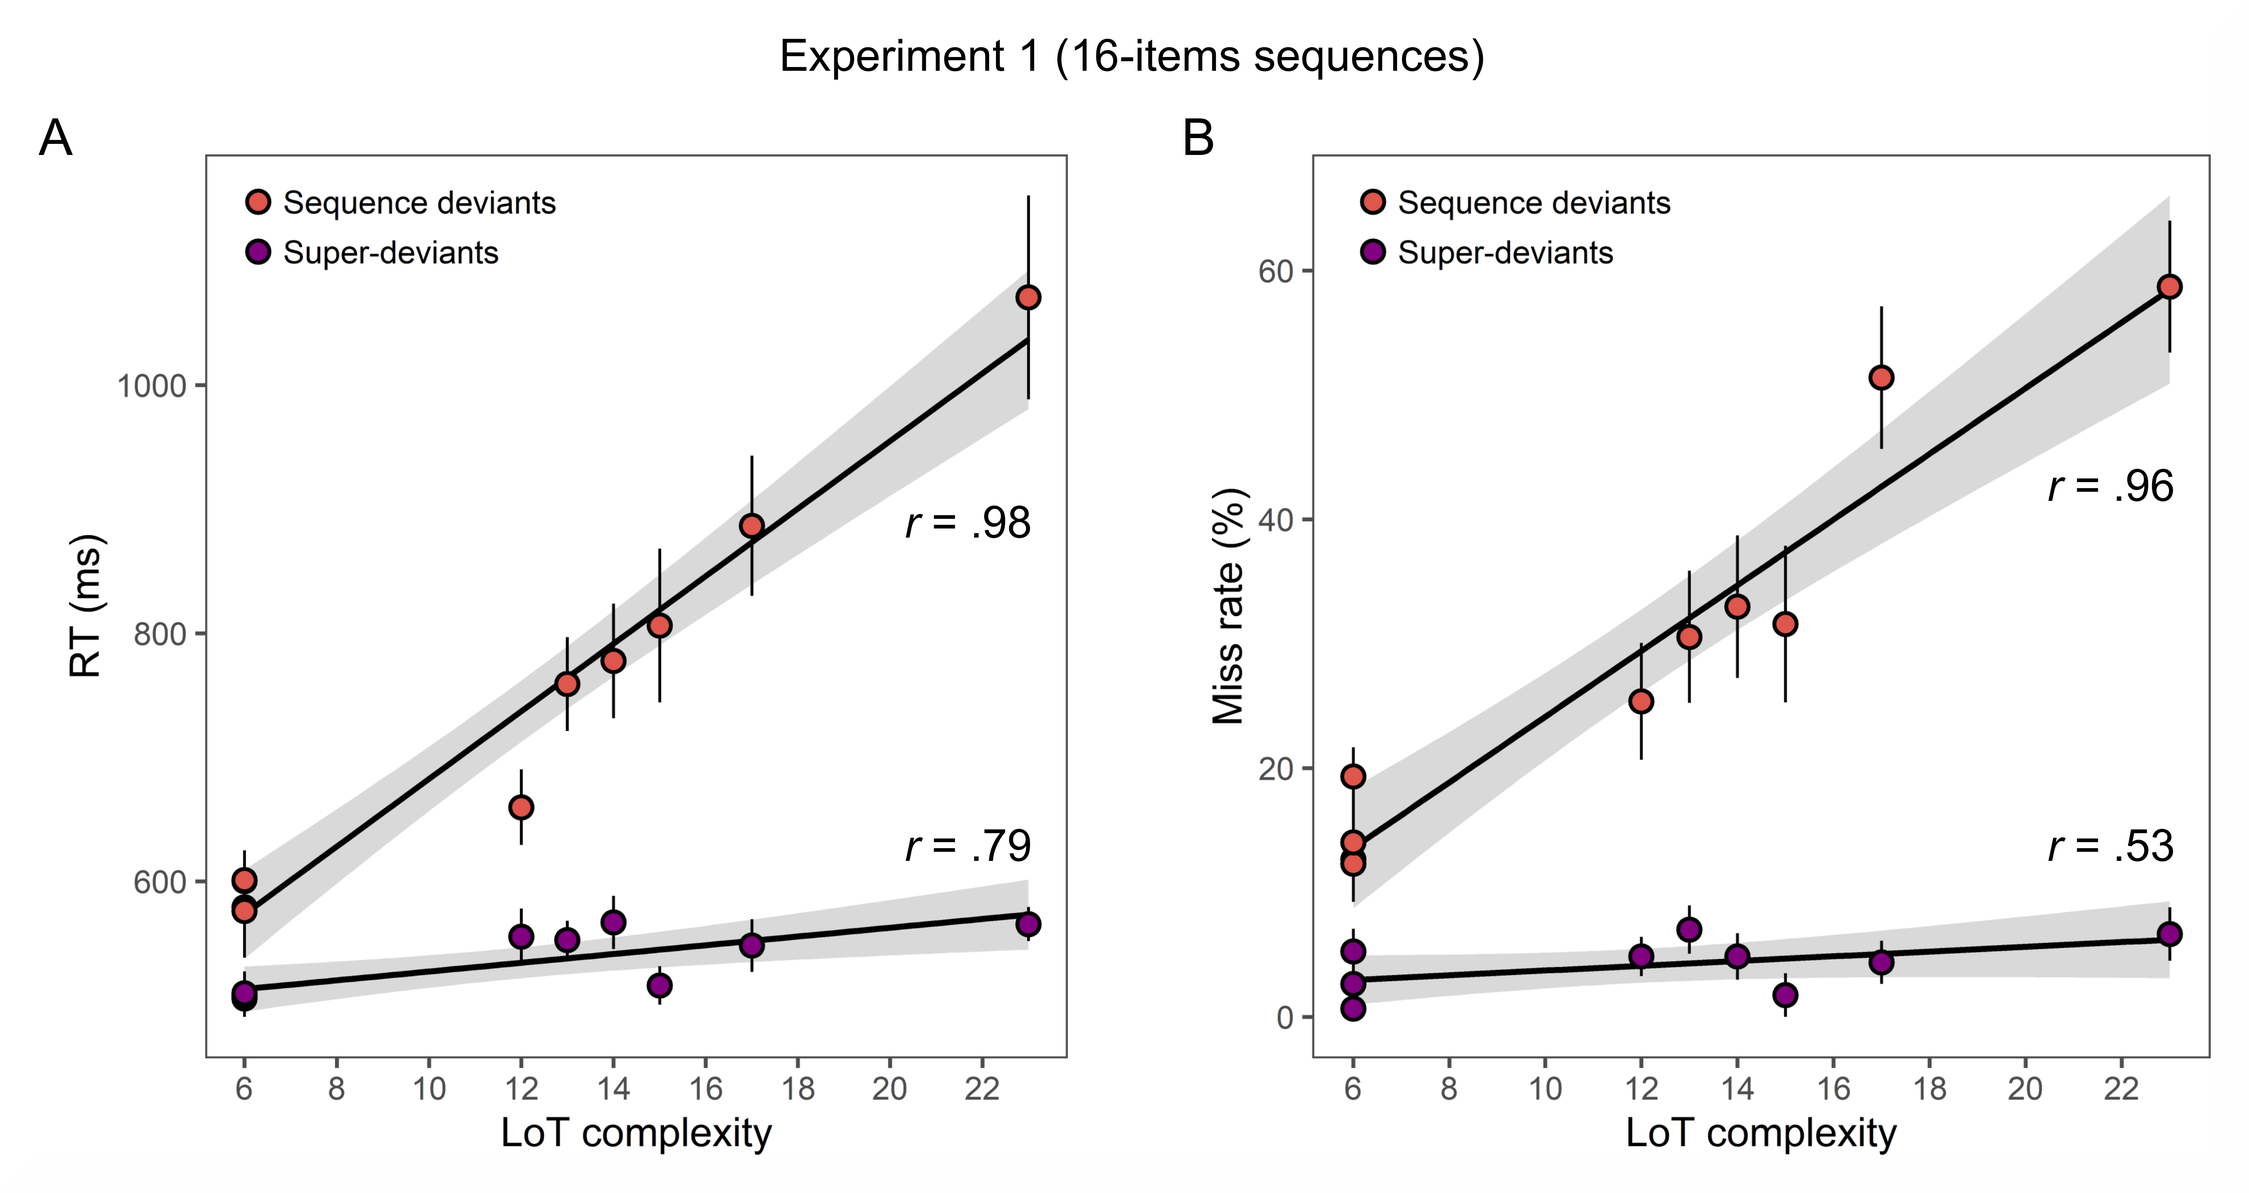
\includegraphics[scale=0.8]{figuras/plosbio/journal.pcbi.1008598.s001.png}
      \centering
      \caption{Relación lineal entre el desempeño de la tarea y \mdlbin en el Experimento 1. A) Tiempo de respuesta promedio y B) Tasa promedio de fallas}
      \label{PlosBIO-S1}
\end{figure}

\begin{figure}[t!]
      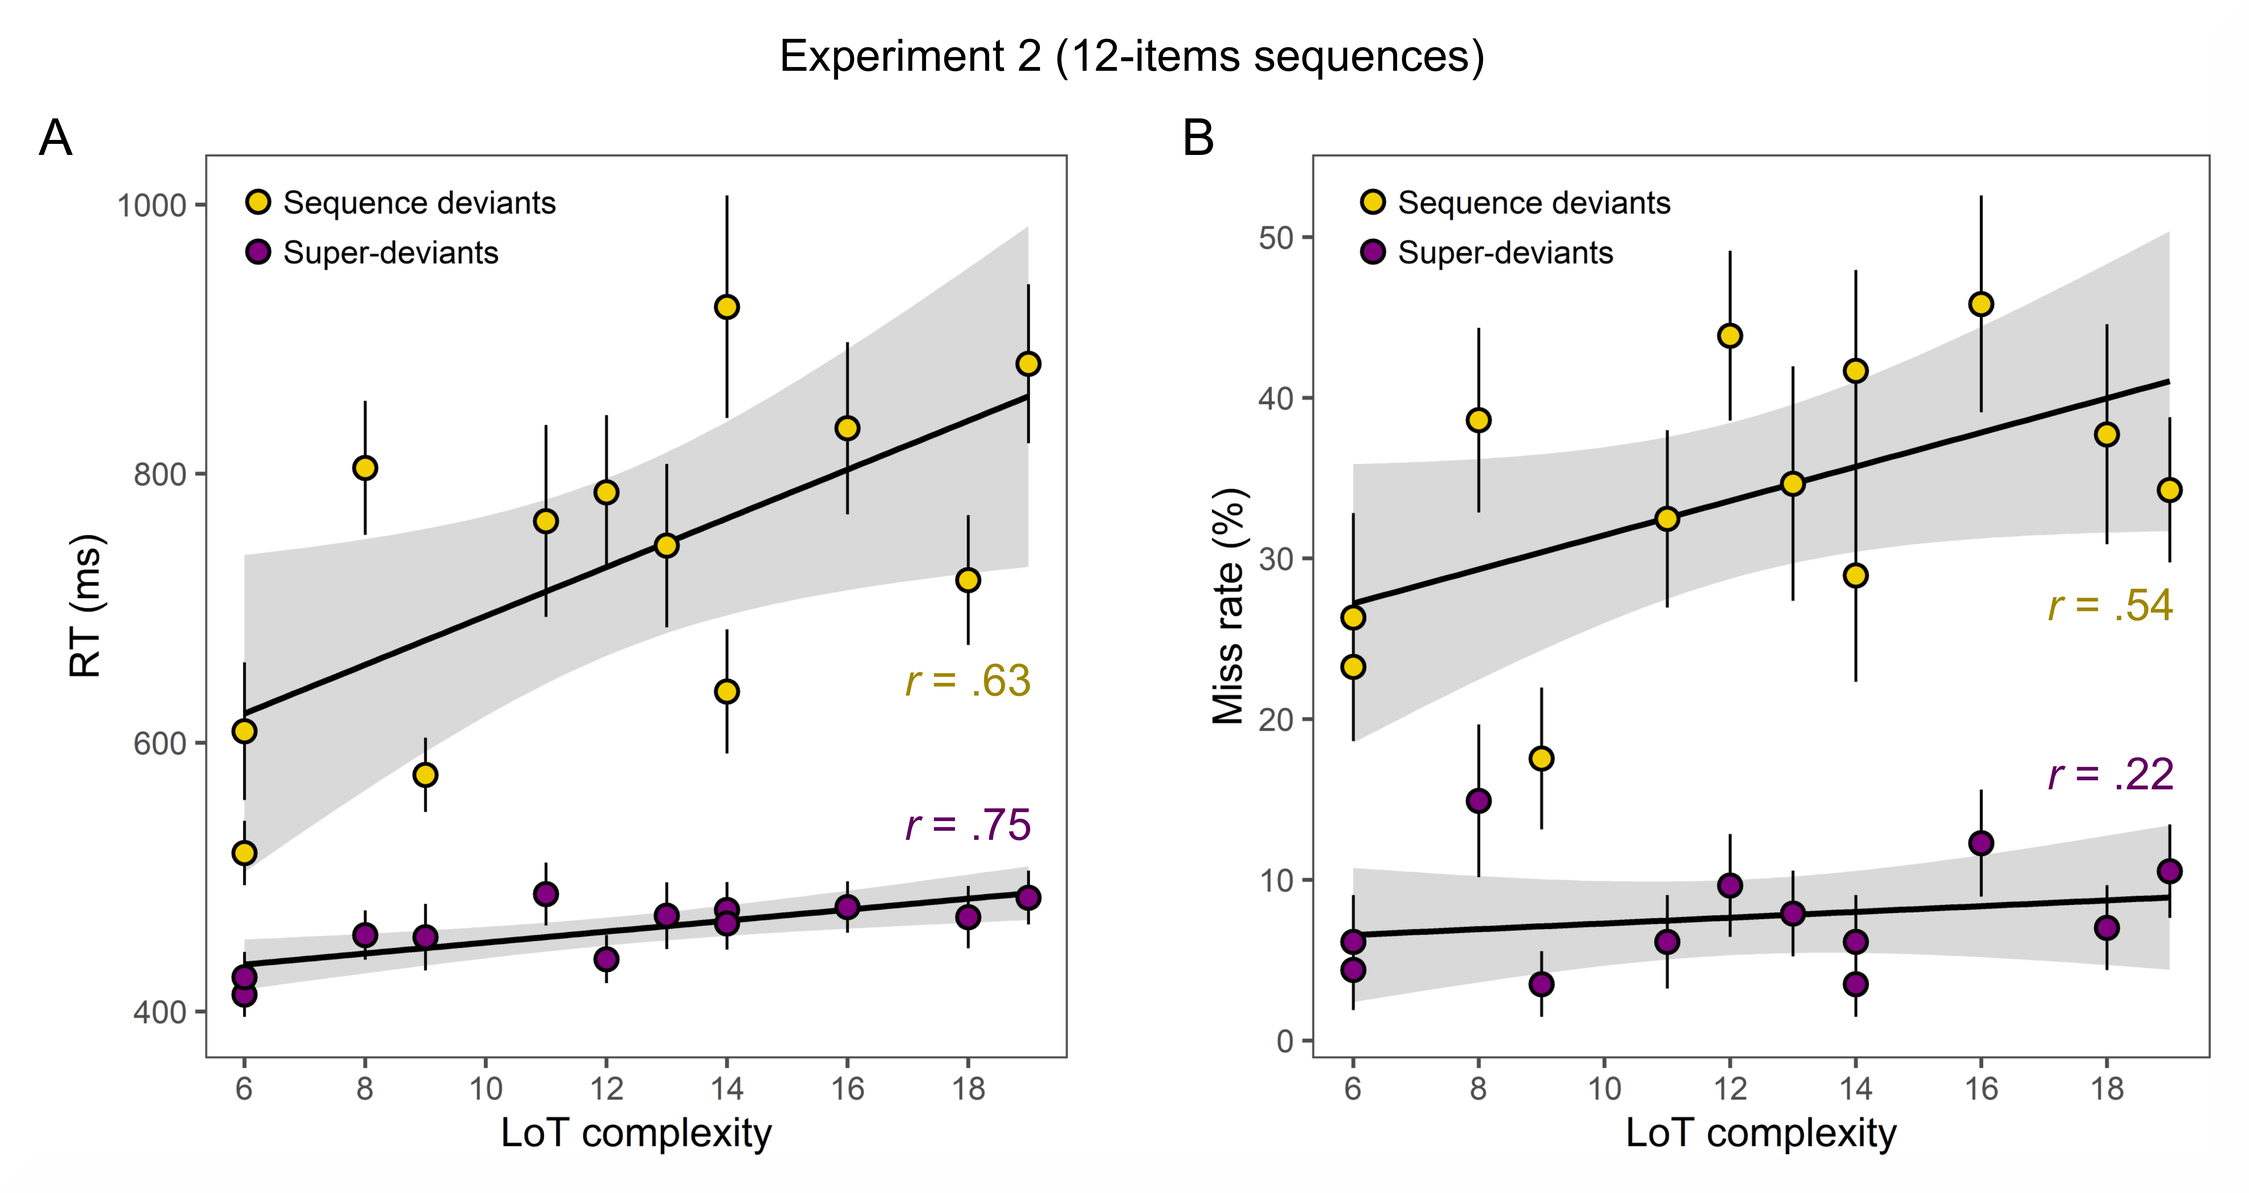
\includegraphics[scale=0.8]{figuras/plosbio/journal.pcbi.1008598.s002.png}
      \centering
      \caption{Relación lineal entre el desempeño de la tarea y \mdlbin en el Experimento 2. A) Tiempo de respuesta promedio y B) Tasa promedio de fallas}
      \label{PlosBIO-S2}
\end{figure}

\begin{figure}[t!]
      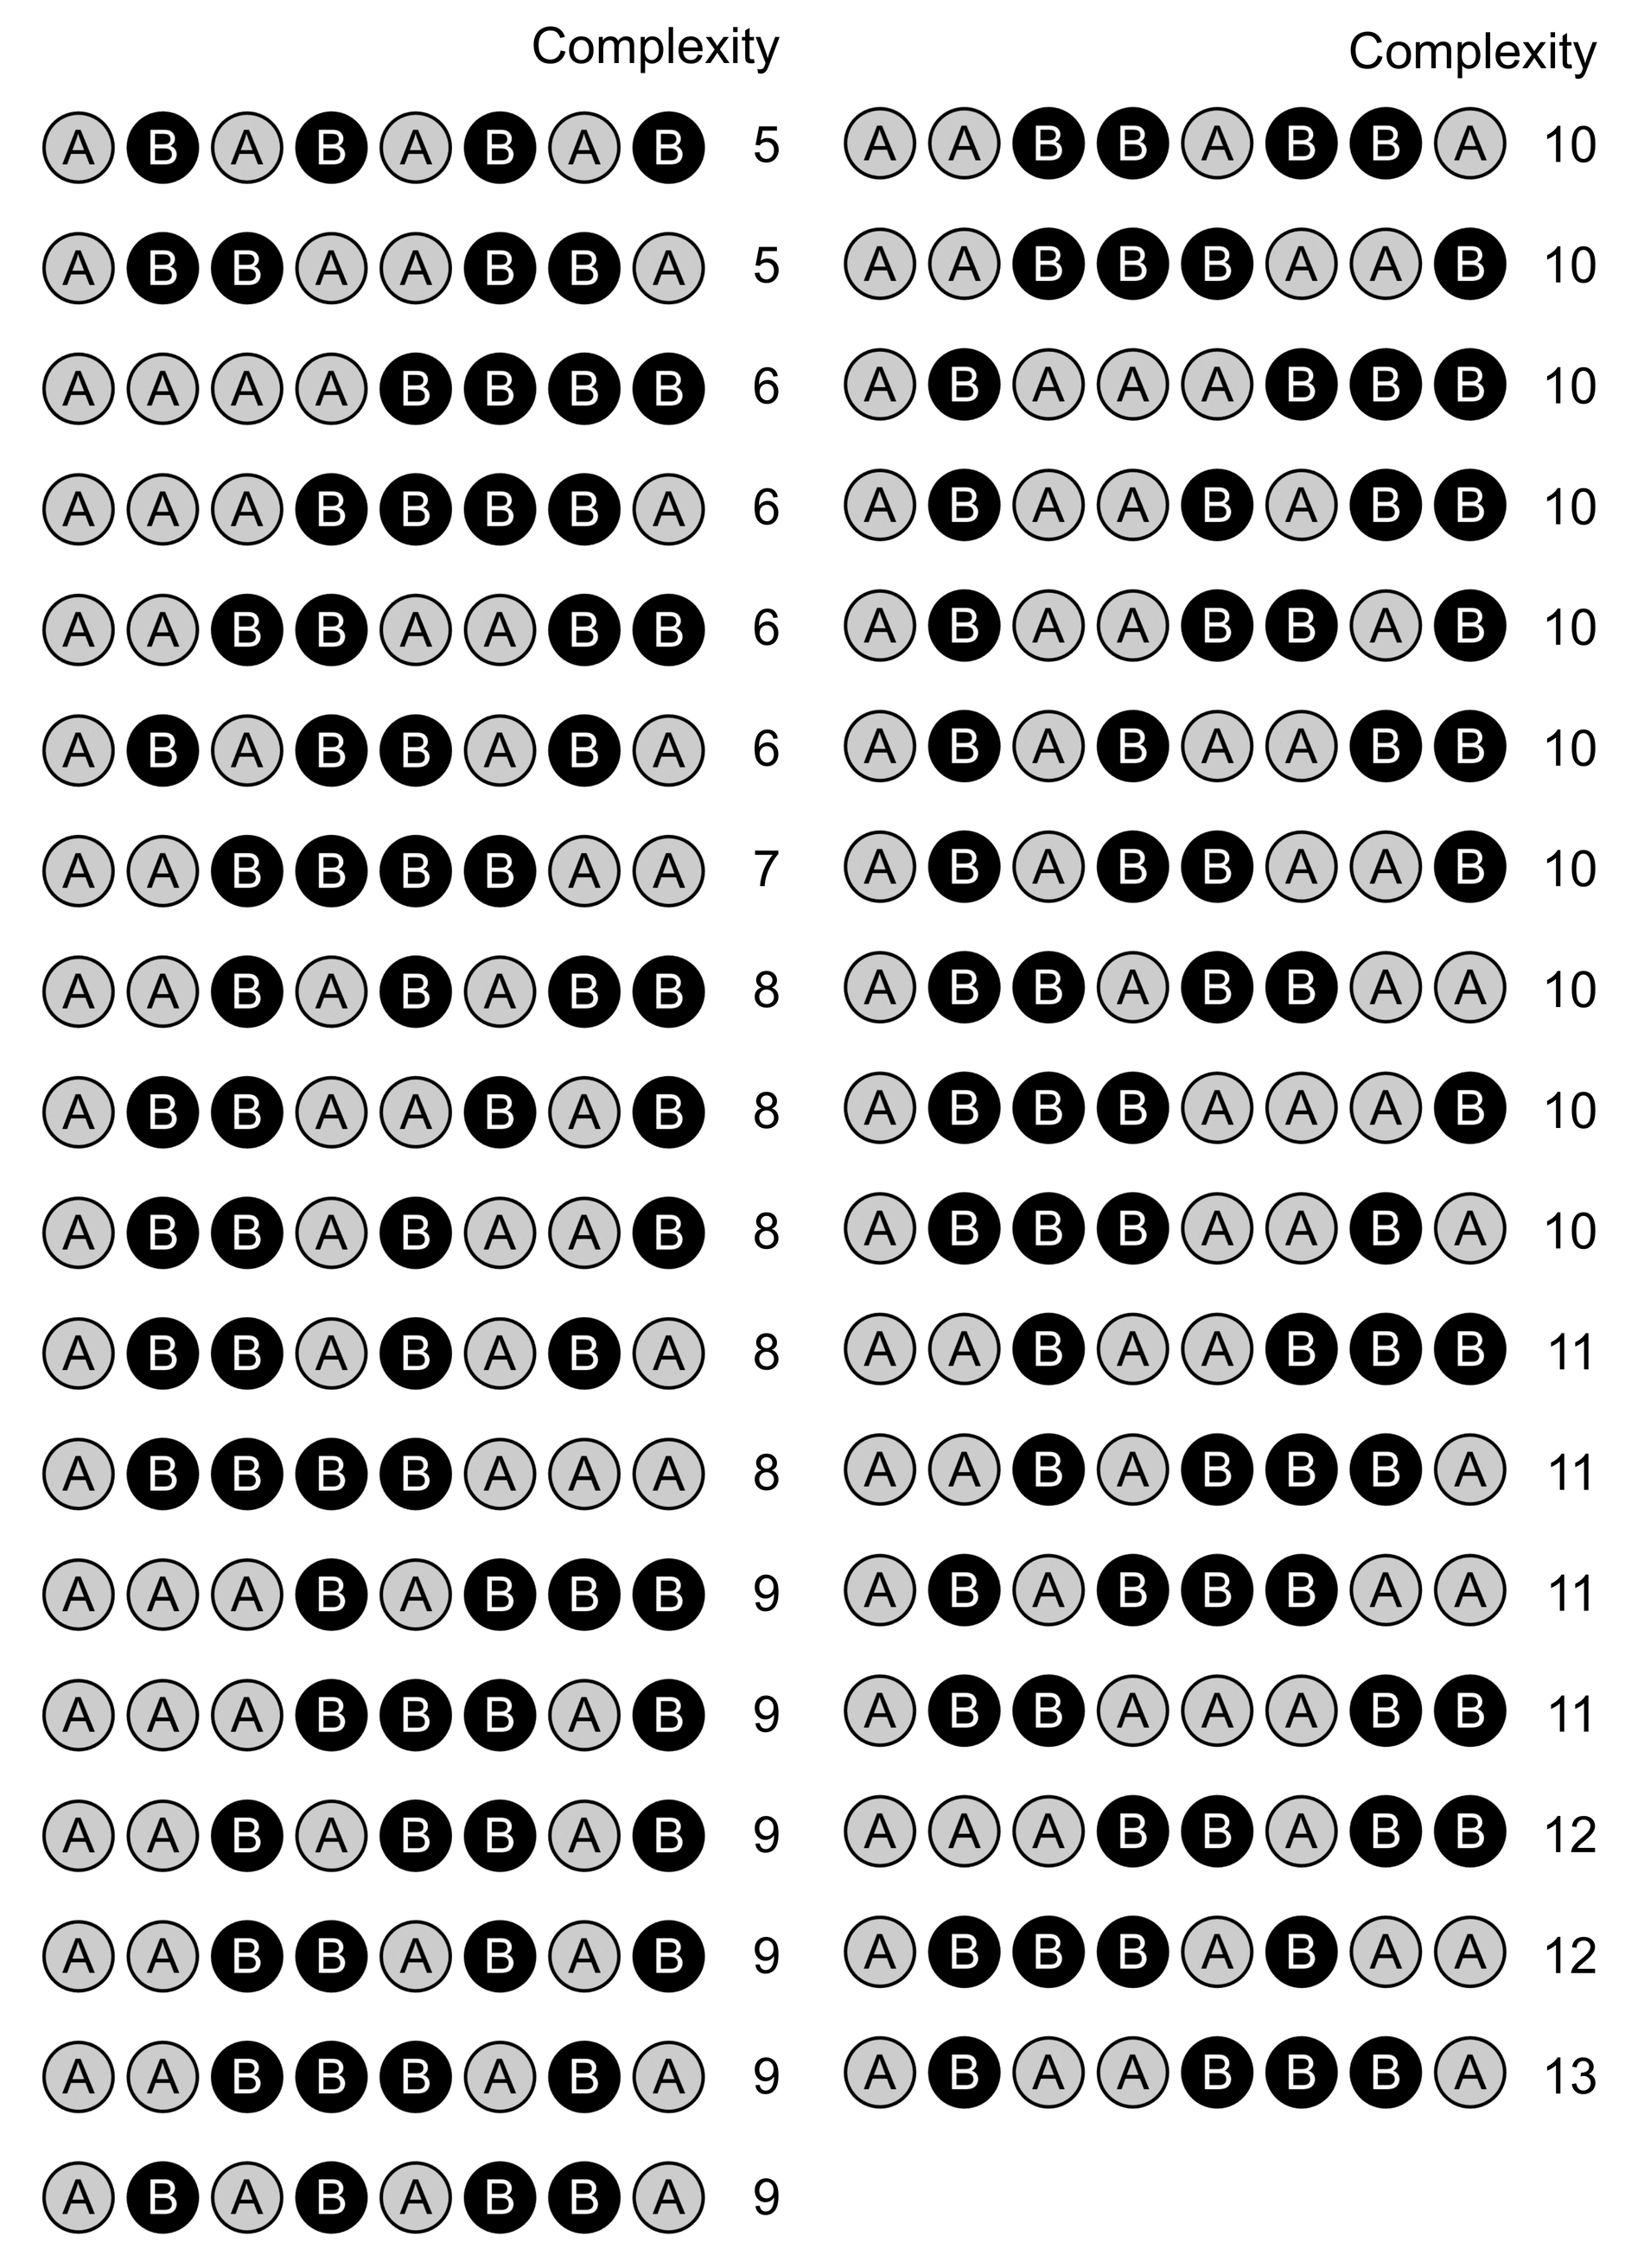
\includegraphics[scale=0.8]{figuras/plosbio/journal.pcbi.1008598.s003.png}
      \centering
      \caption{Secuencias utilizadas en el Experimento 3}
      \label{PlosBIO-S3}
\end{figure}

\begin{figure}[t!]
      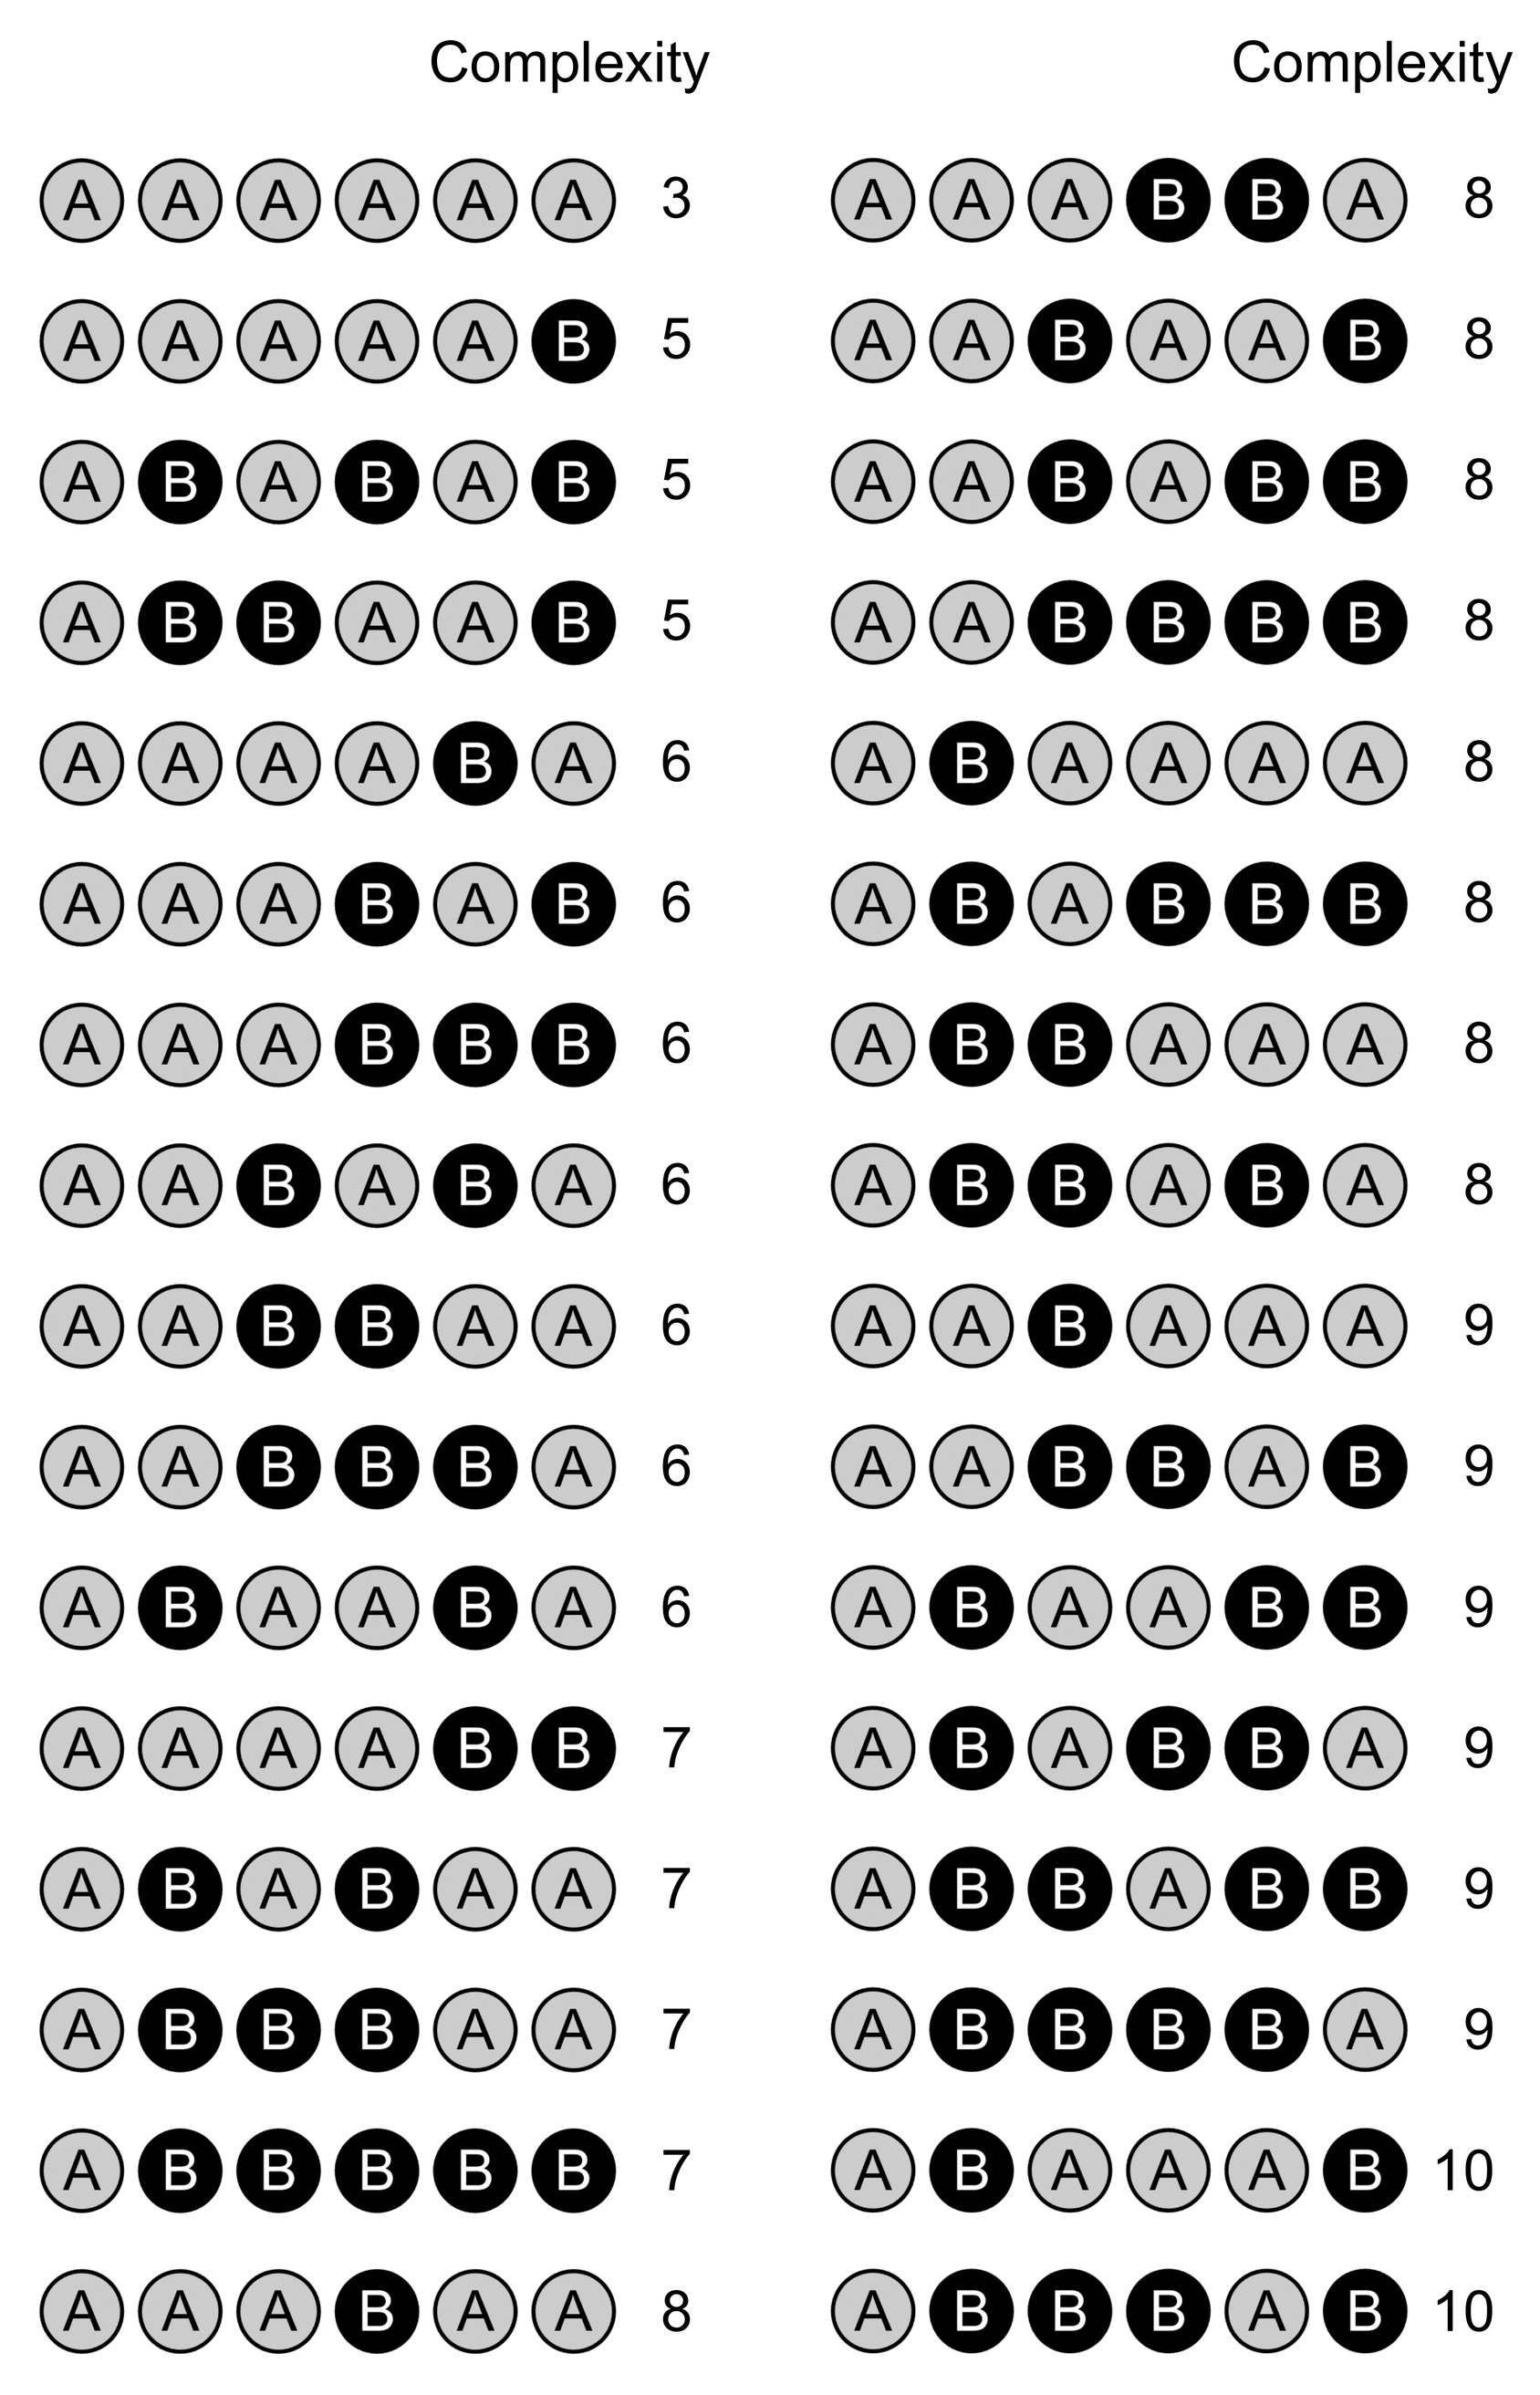
\includegraphics[scale=0.8]{figuras/plosbio/journal.pcbi.1008598.s004.png}
      \centering
      \caption{Secuencias utilizadas en el Experimento 4}
      \label{PlosBIO-S4}
\end{figure}

\begin{figure}[t!]
      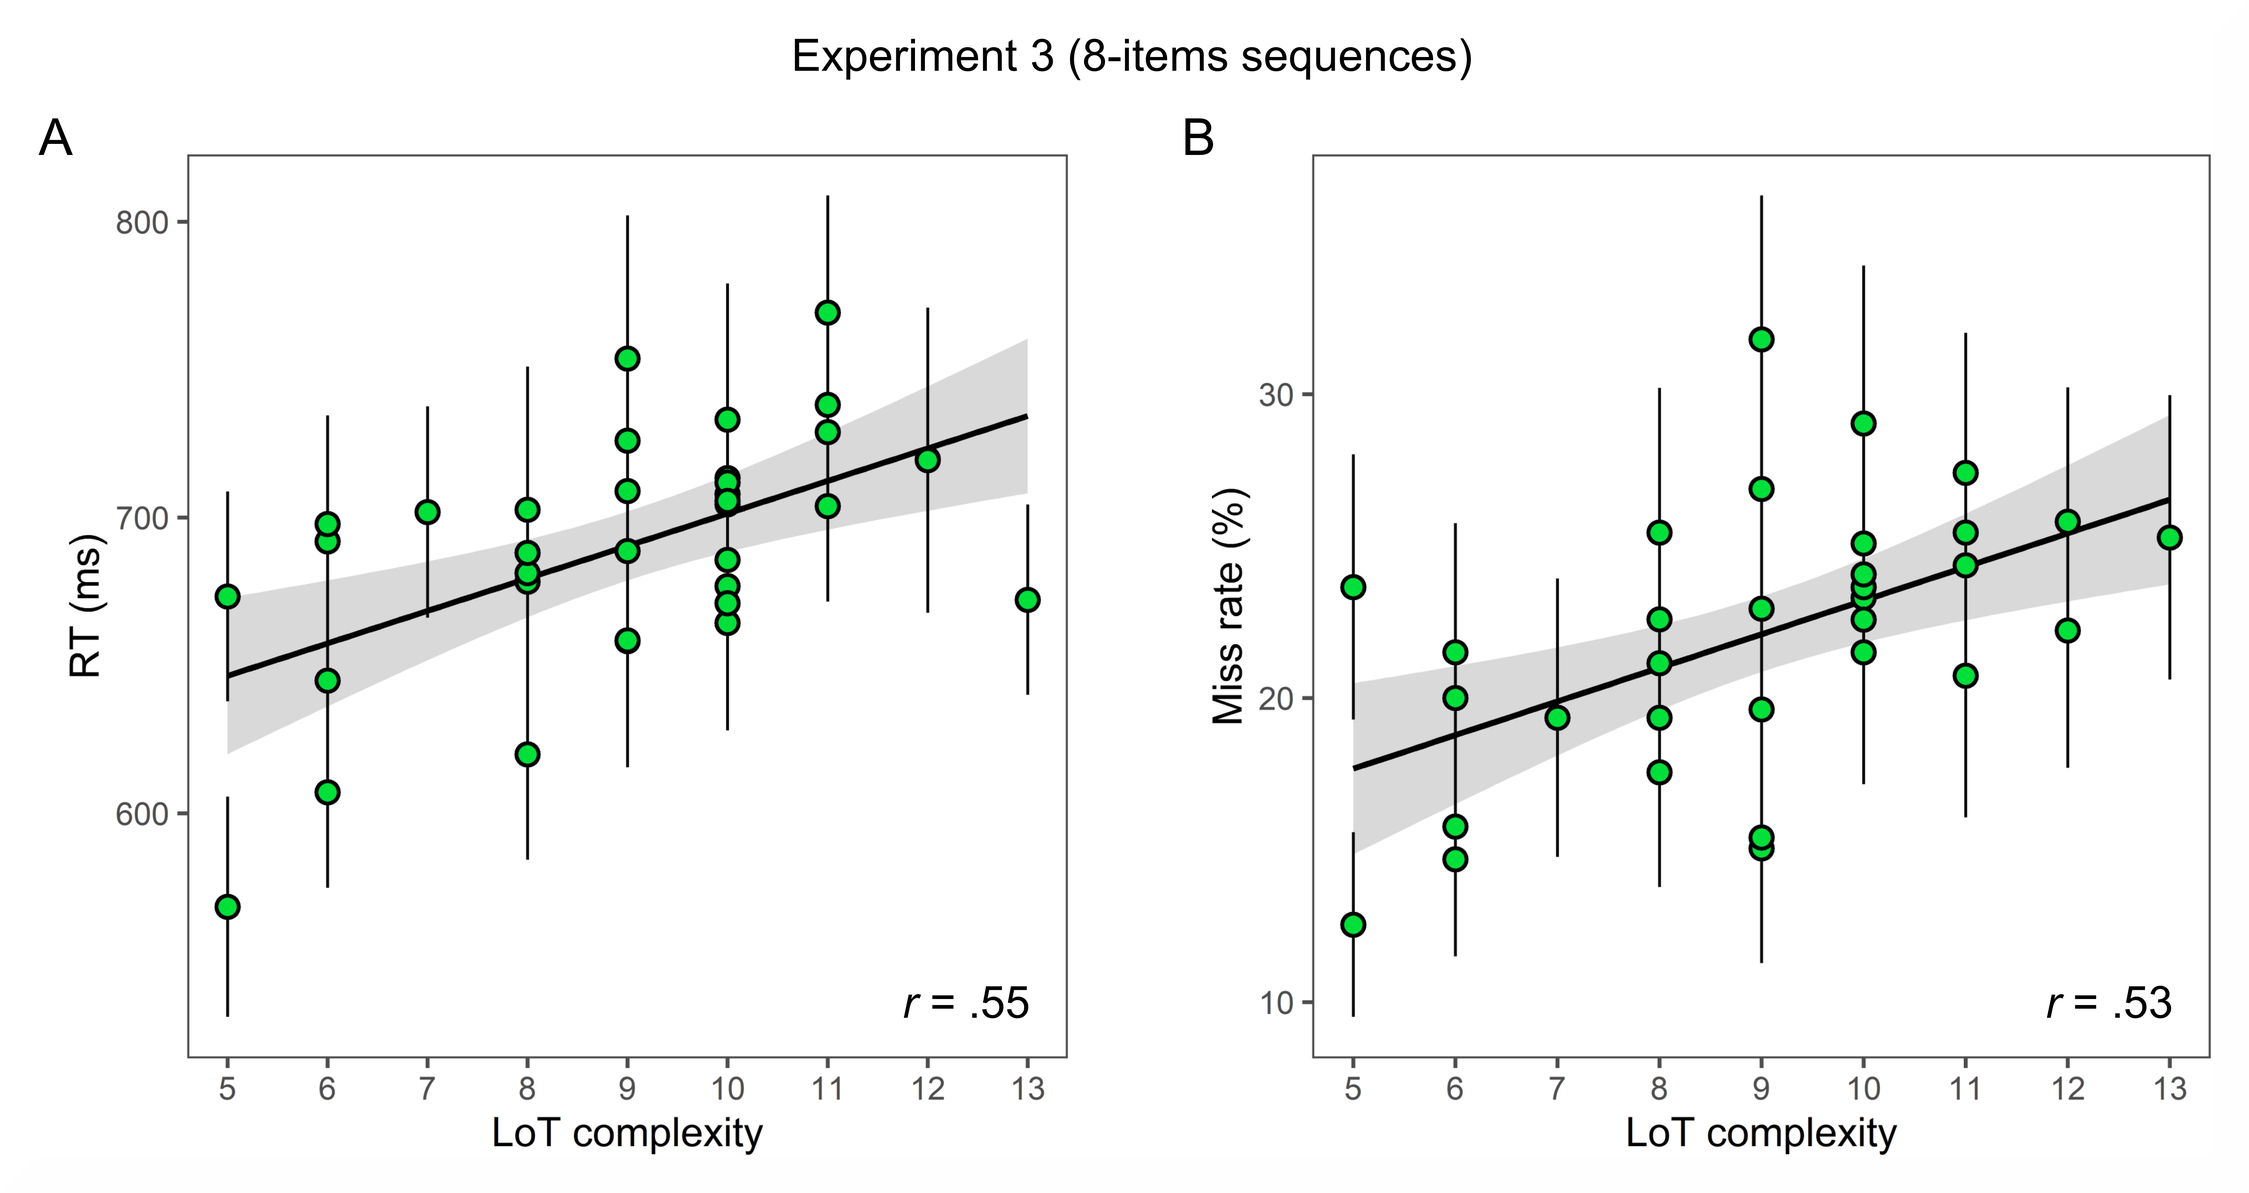
\includegraphics[scale=0.8]{figuras/plosbio/journal.pcbi.1008598.s005.png}
      \centering
      \caption{Relación lineal entre el desempeño de la tarea y \mdlbin en el Experimento 3. A) Tiempo de respuesta promedio y B) Tasa promedio de fallas}
      \label{PlosBIO-S5}
\end{figure}

\begin{figure}[t!]
      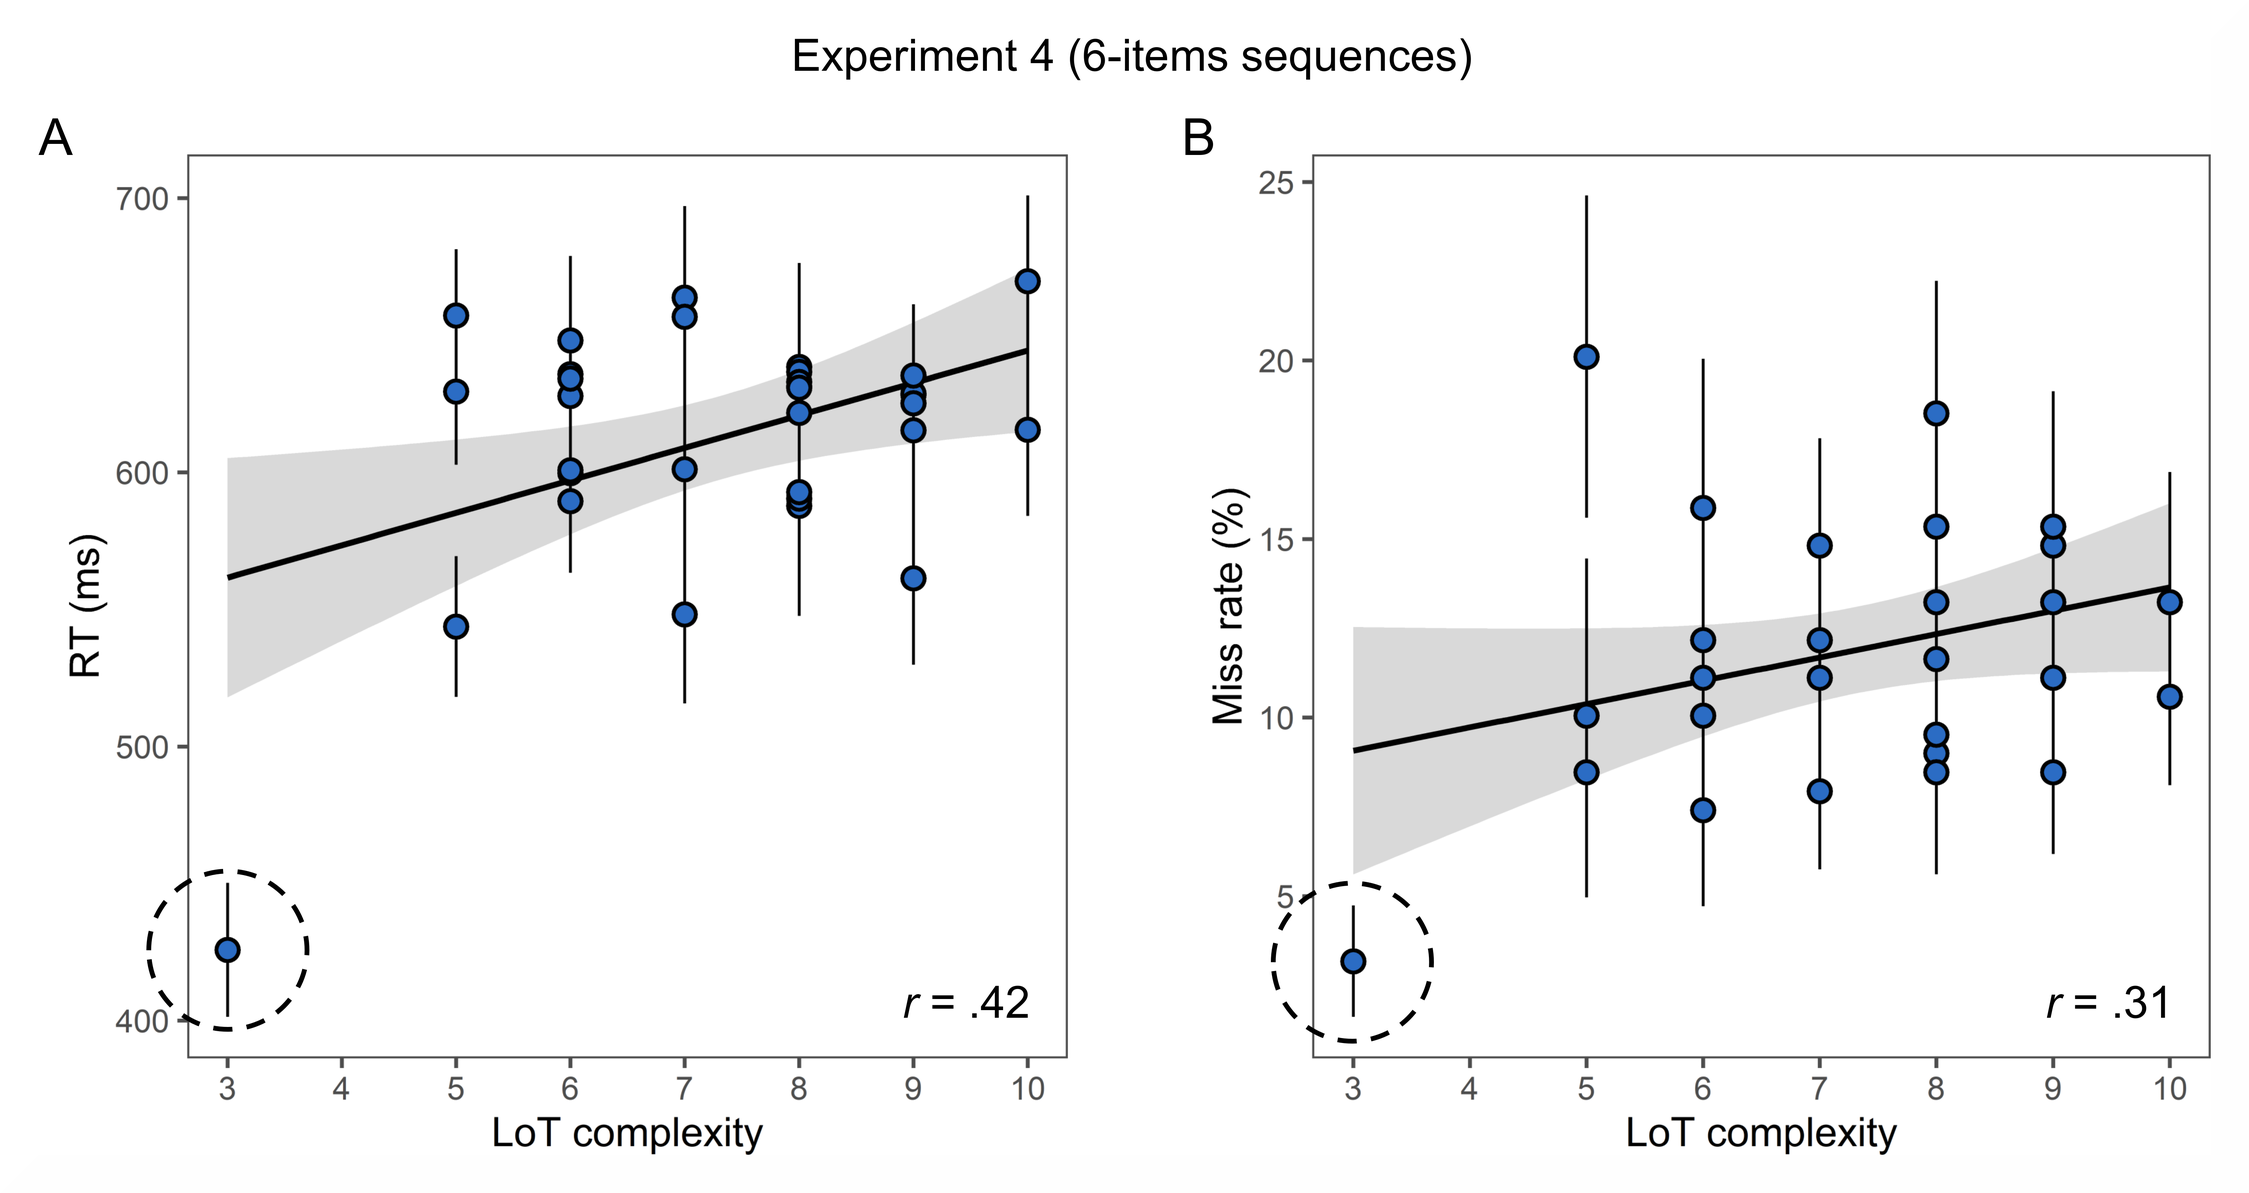
\includegraphics[scale=0.8]{figuras/plosbio/journal.pcbi.1008598.s006.png}
      \centering
      \caption{Relación lineal entre el desempeño de la tarea y \mdlbin en el Experimento 4 . A) Tiempo de respuesta promedio y B) Tasa promedio de fallas. Nota: el punto encerrado en un círculo resalta el desempeño de la secuencia AAAAAA, que fue excluida de algunos análisis}
      \label{PlosBIO-S6}
\end{figure}

\begin{figure}[t!]
      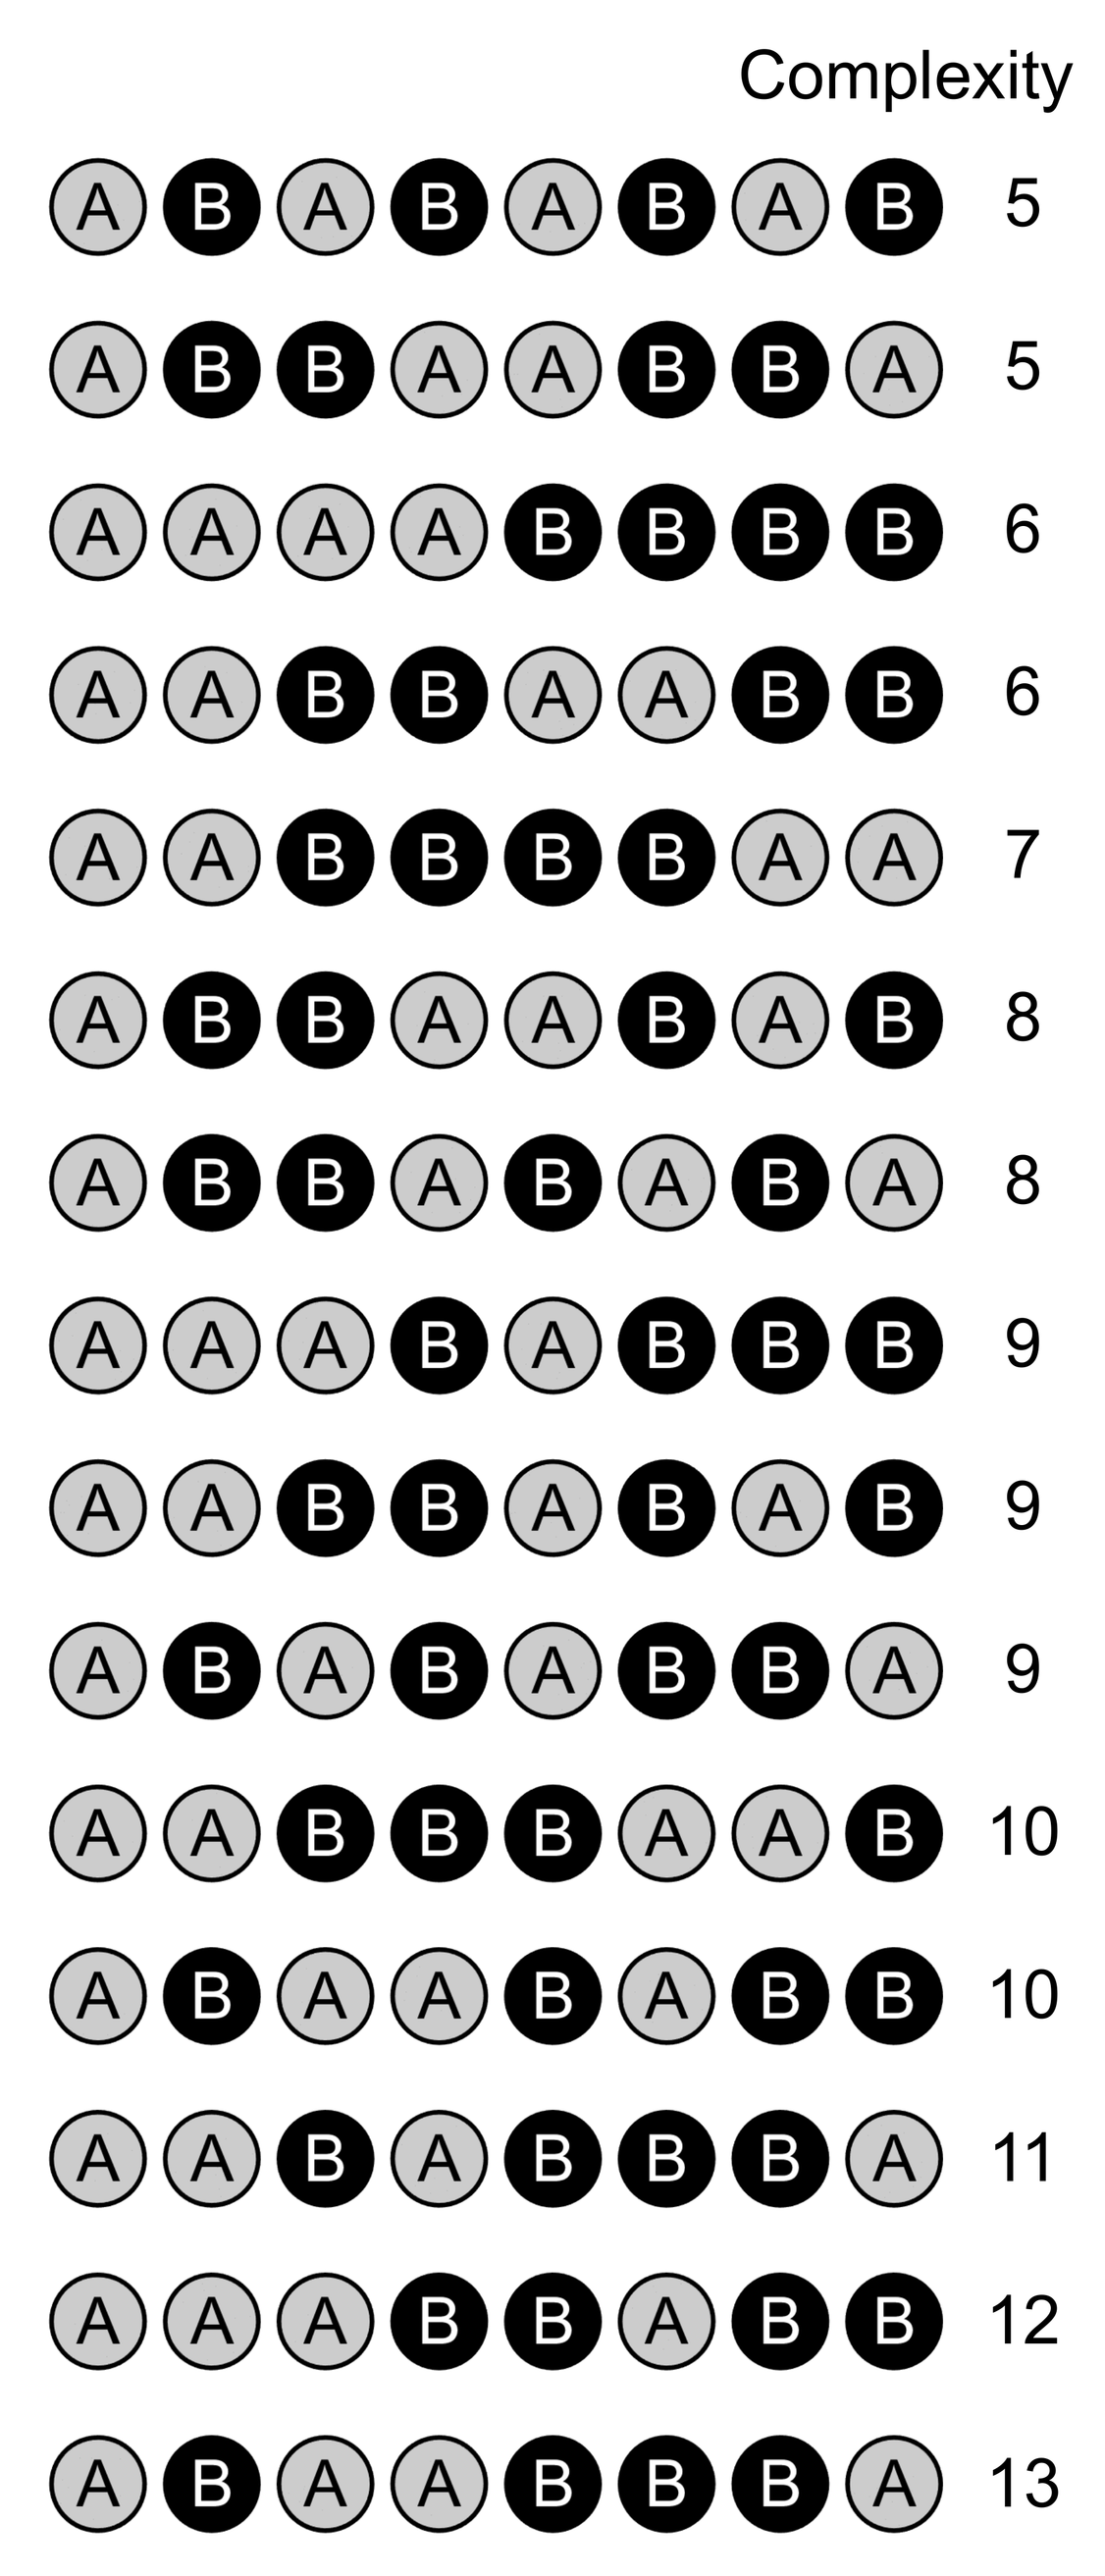
\includegraphics[scale=0.8]{figuras/plosbio/journal.pcbi.1008598.s007.png}
      \centering
      \caption{Secuencias utilizadas en el Experimento 5}
      \label{PlosBIO-S7}
\end{figure}

\begin{figure}[t!]
      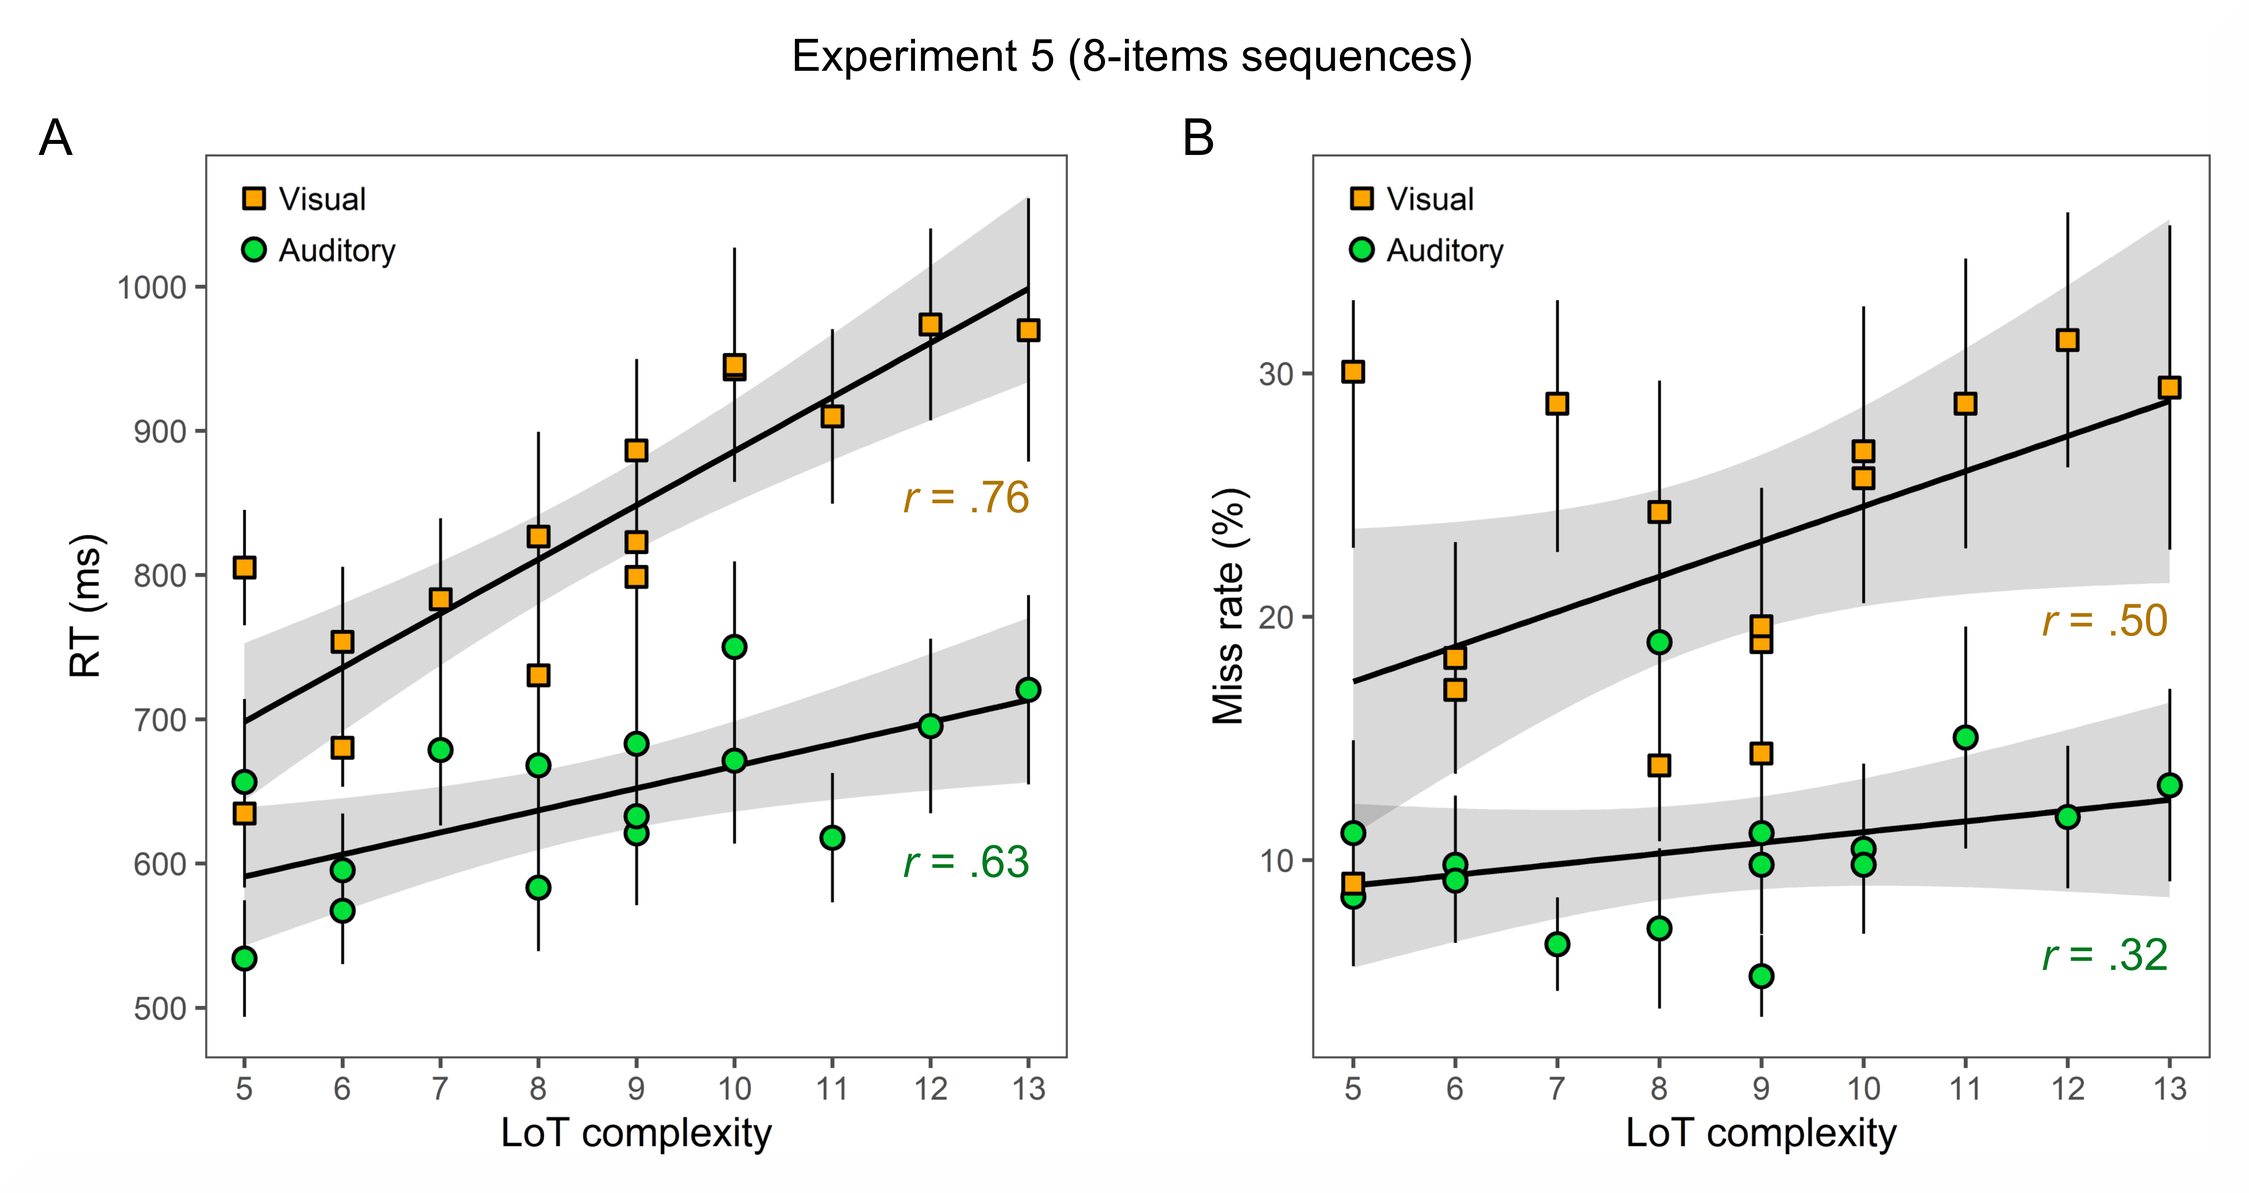
\includegraphics[scale=0.8]{figuras/plosbio/journal.pcbi.1008598.s008.png}
      \centering
      \caption{Relación lineal entre el desempeño de la tarea y \mdlbin en el Experimento 5. A) Tiempo de respuesta promedio y B) Tasa promedio de fallas}
      \label{PlosBIO-S8}
\end{figure}

\begin{figure}[t!]
      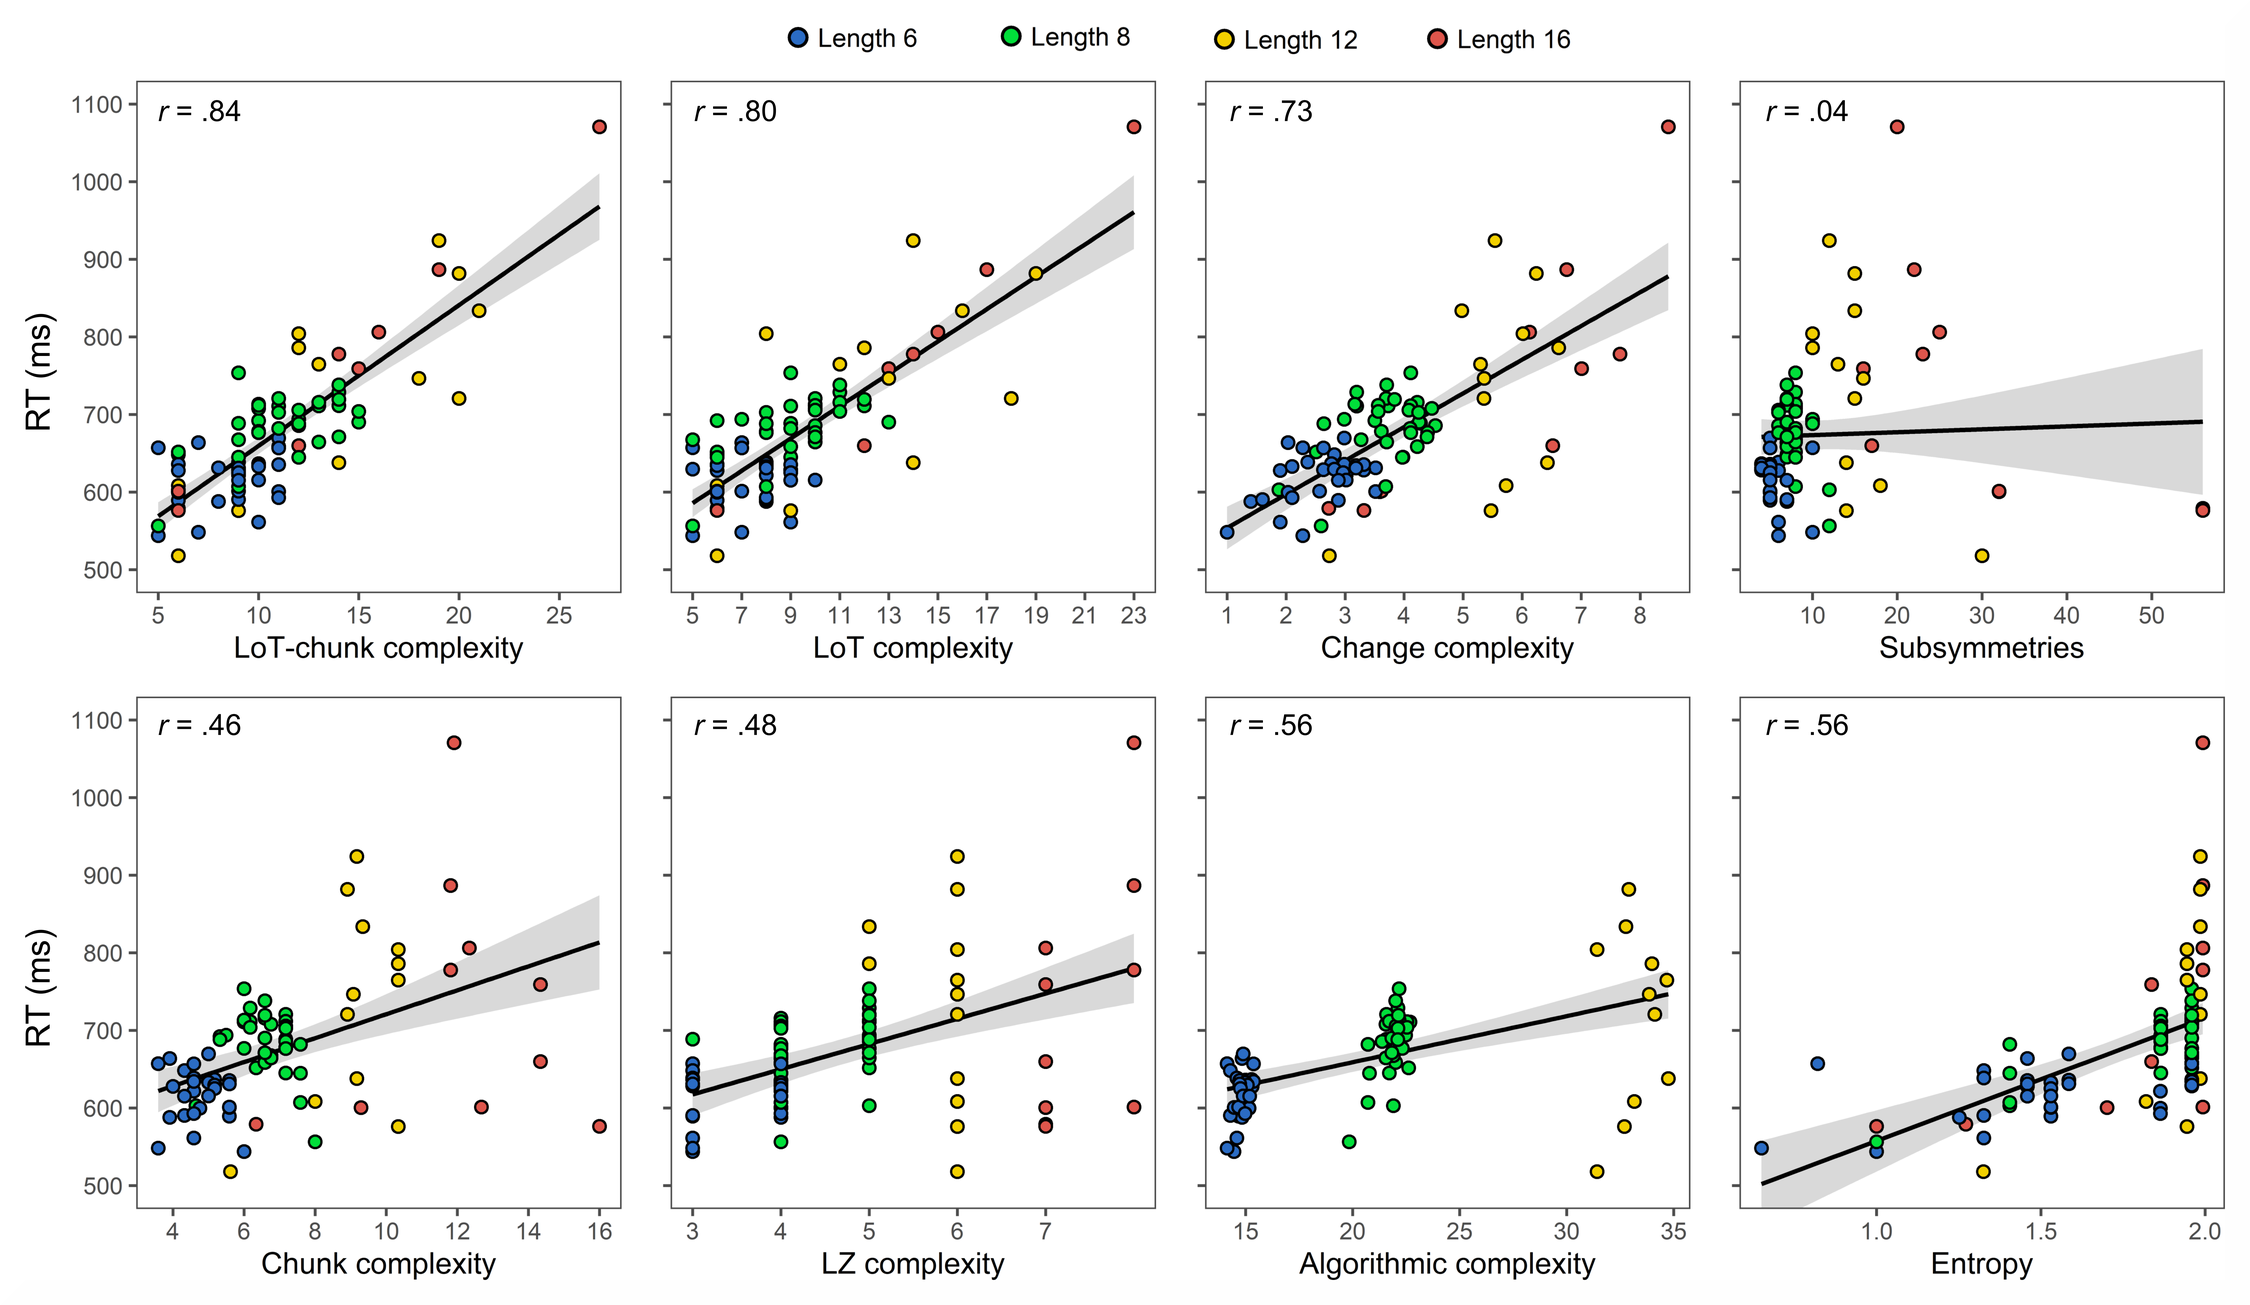
\includegraphics[scale=0.8]{figuras/plosbio/journal.pcbi.1008598.s009.png}
      \centering
      \caption{ Regresiones lineales del tiempo de respuesta promedio (RT) por secuencia (en ms) con ocho predictores diferentes de interés (cuando se combinaron los datos de experimentos con secuencias auditivas de 4 longitudes diferentes). Nota: Las secuencias largas de 16 elementos (así como una secuencia de 12 elementos) no se pudieron incluir en la regresión con complejidad algorítmica}
      \label{PlosBIO-S9}
\end{figure}

\begin{figure}[t!]
      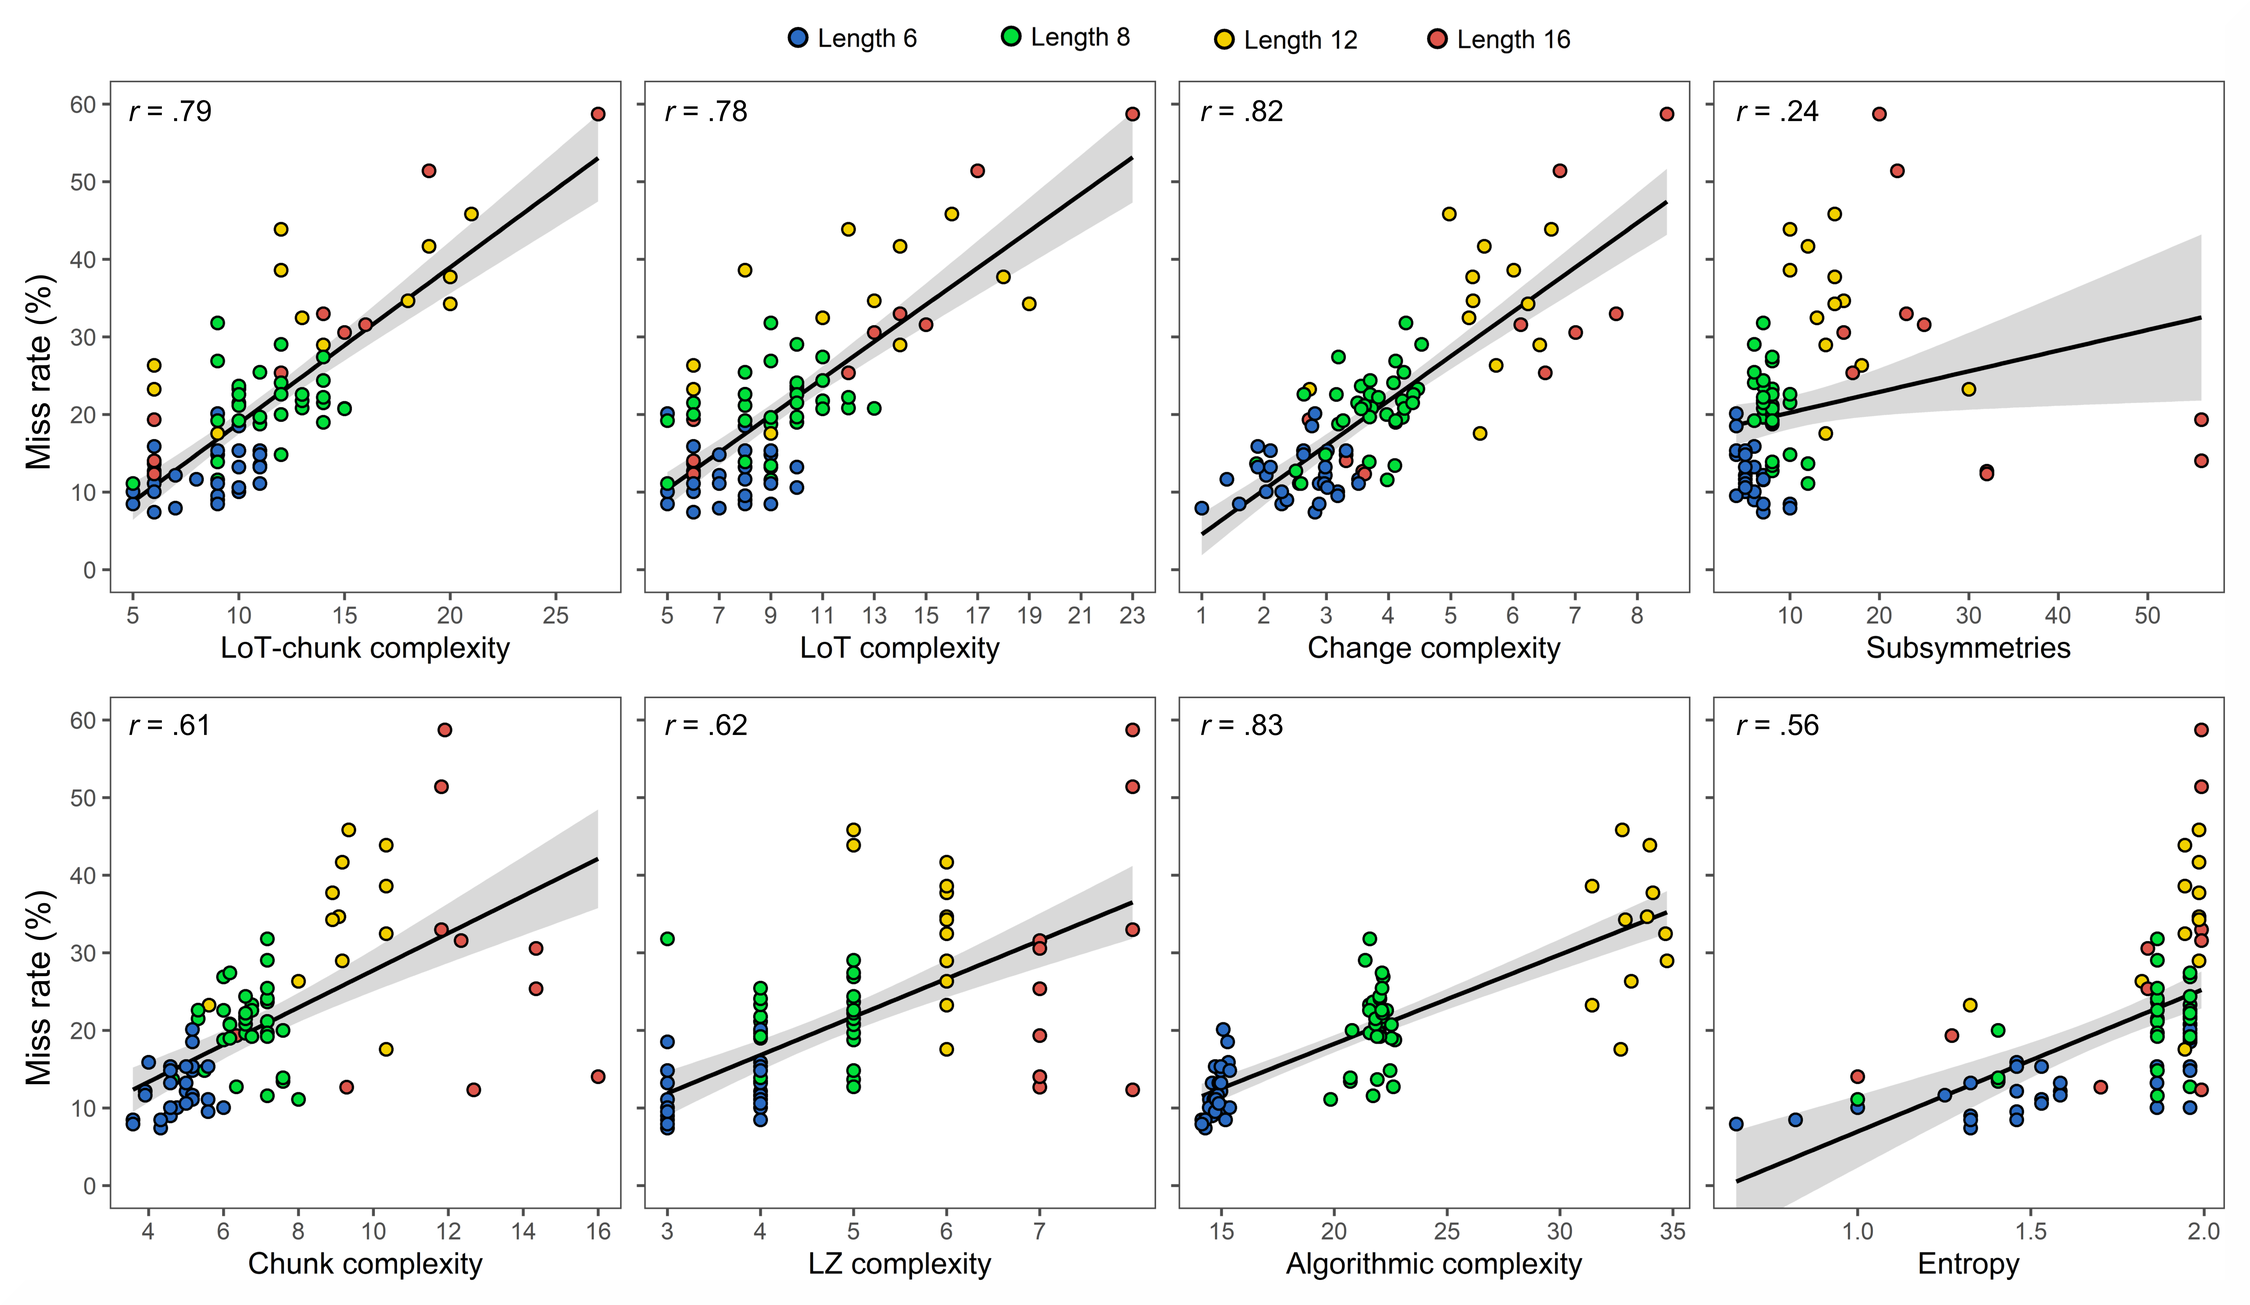
\includegraphics[scale=0.8]{figuras/plosbio/journal.pcbi.1008598.s010.png}
      \centering
      \caption{Regresiones lineales de la tasa de aciertos promedio por secuencia (en \%) con ocho predictores de interés diferentes (cuando se combinaron los datos de experimentos con secuencias auditivas de 4 longitudes diferentes)}
      \label{PlosBIO-S10}
\end{figure}

\begin{figure}[t!]
      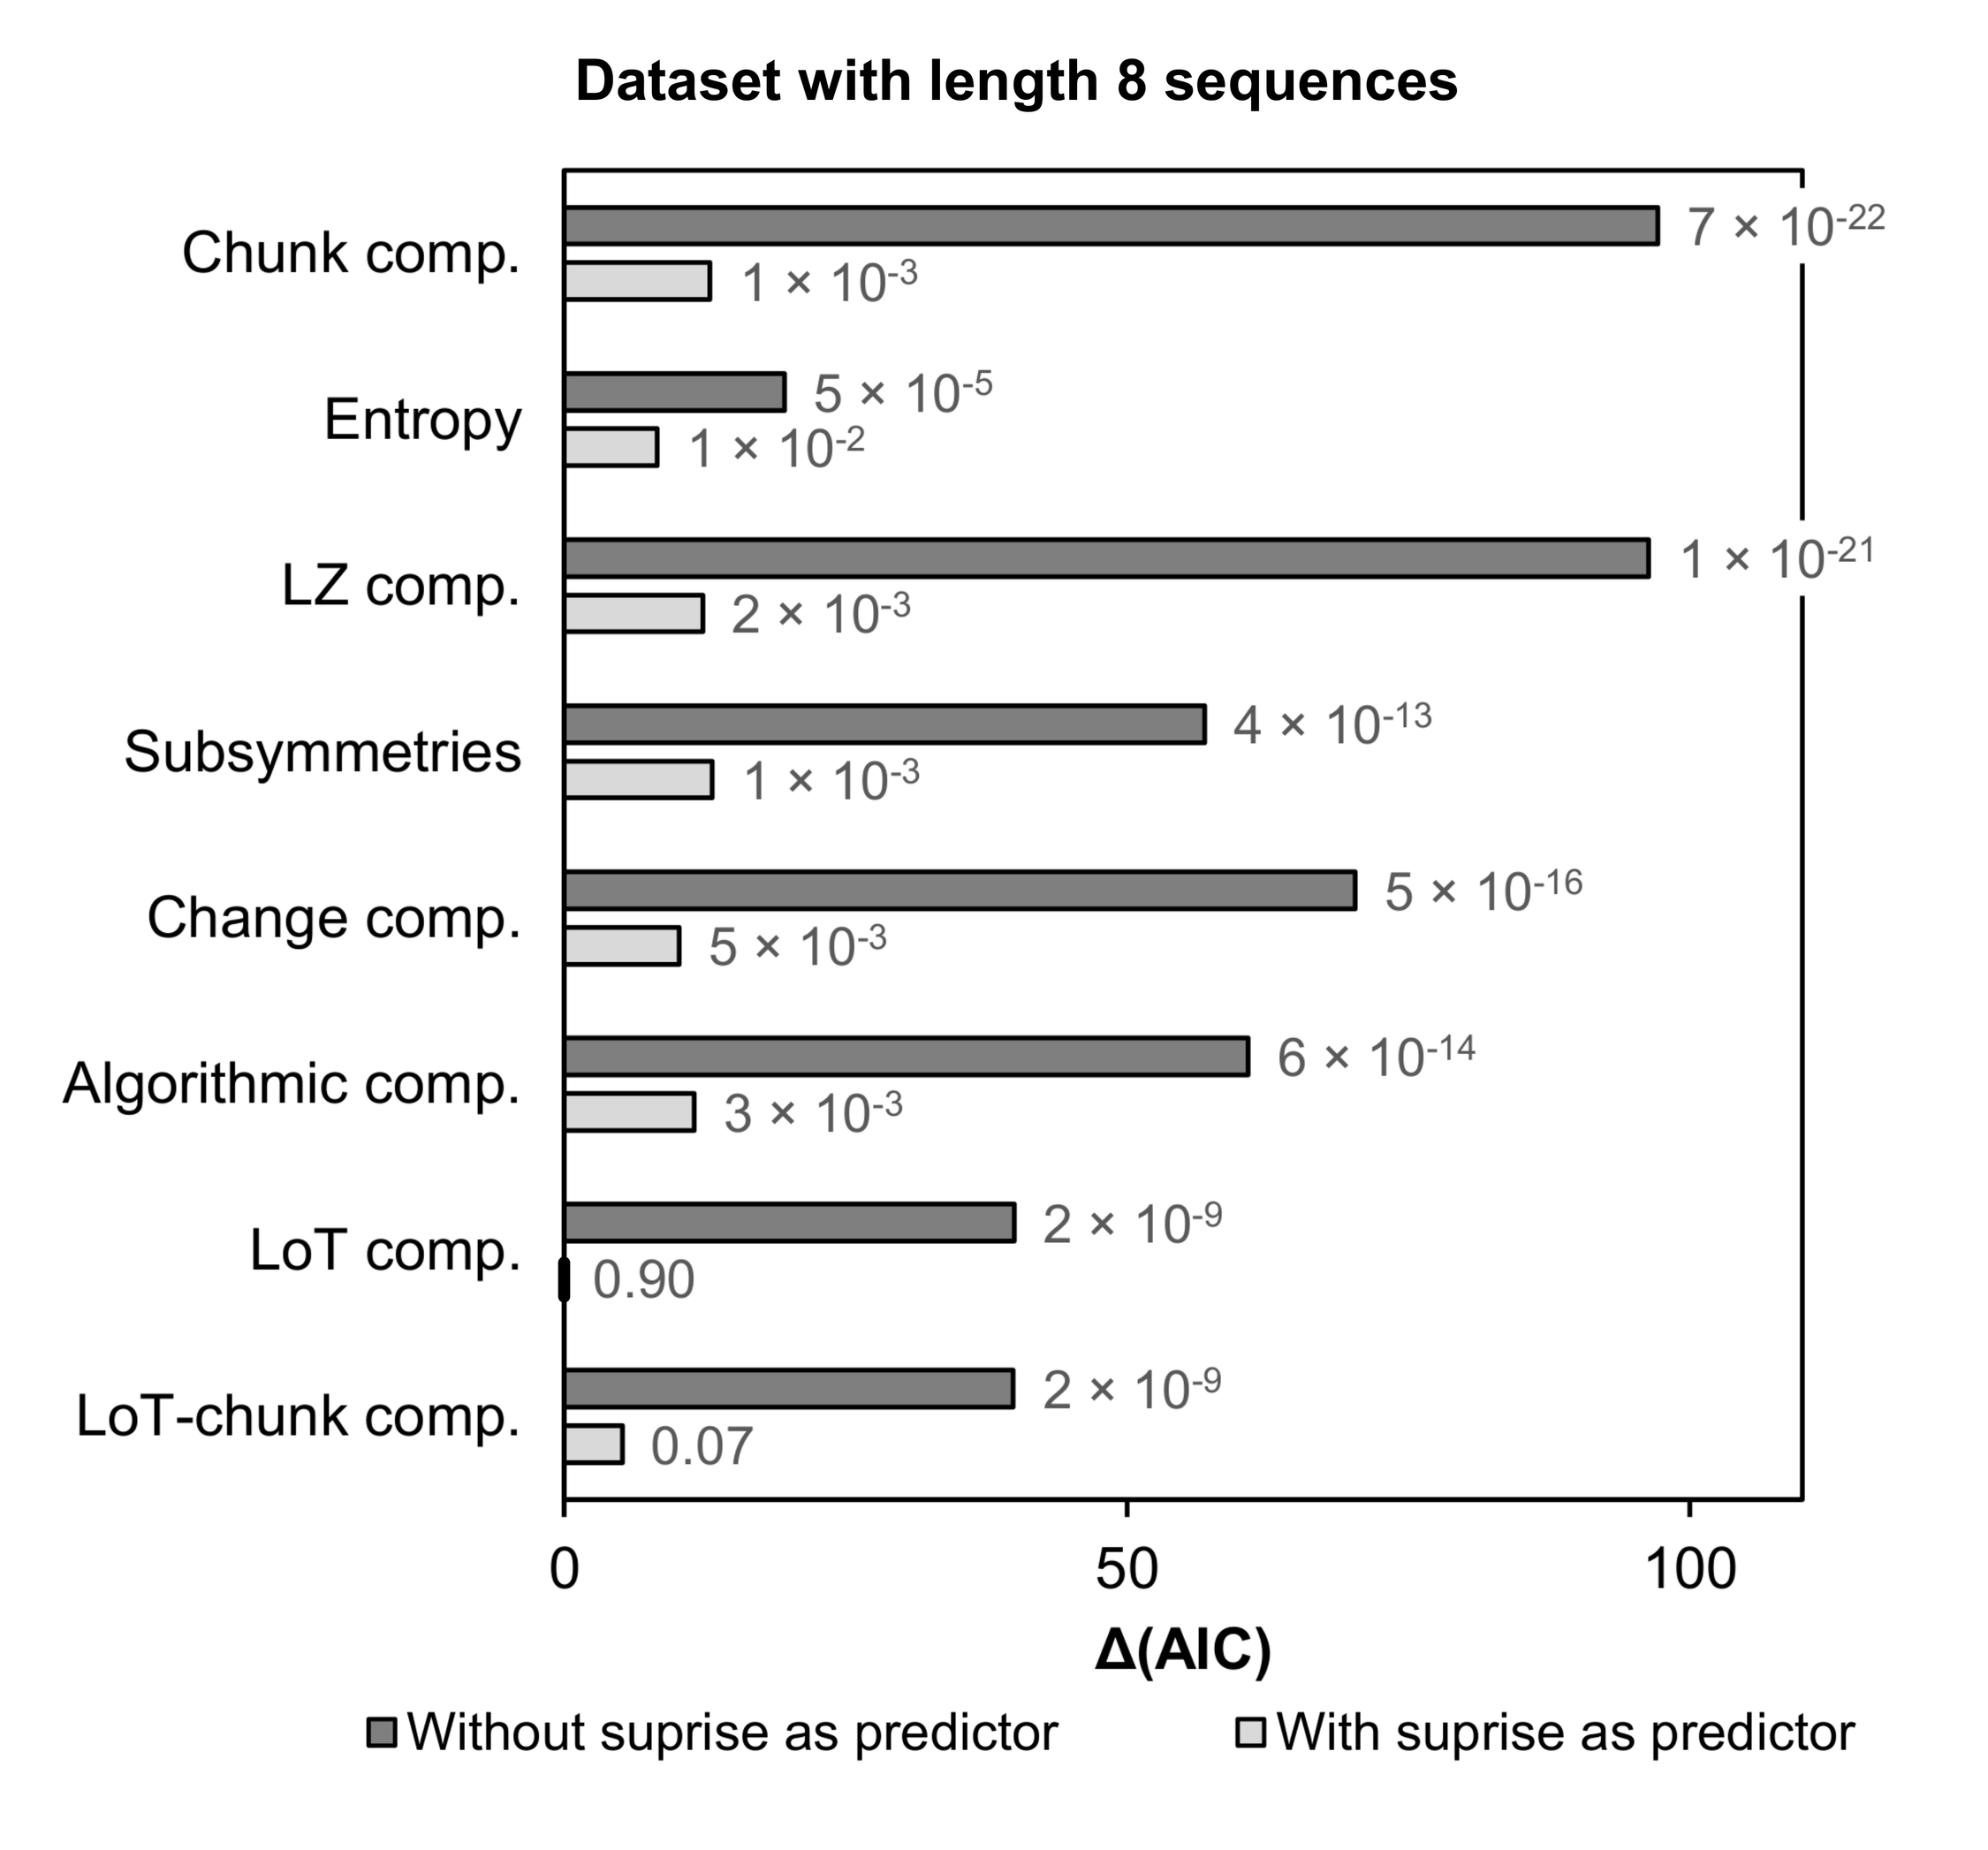
\includegraphics[scale=0.8]{figuras/plosbio/journal.pcbi.1008598.s011.png}
      \centering
      \caption{Comparación del modelo mixto complementario con secuencias de longitud 8. $\Delta$ (AIC) para los dieciséis modelos mixtos probados utilizando un conjunto de datos que incluye el rendimiento de la tarea (LISAS) para secuencias de longitud 8 (35 secuencias). El efecto fijo de interés se indica a lo largo del eje vertical (todos los modelos incluyeron a los participantes como un efecto aleatorio y podrían incluir la sorpresa como una covariable: barras de color gris claro). También se informa el peso Akaike para cada modelo}
      \label{PlosBIO-S11}
\end{figure}